\documentclass[11pt,a4paper]{article}
\usepackage[utf8]{inputenc}
\usepackage[italian]{babel}
\usepackage{amsmath}
\usepackage{amsfonts}
\usepackage{amssymb}
\usepackage{array}
\usepackage{graphicx}
\usepackage{multirow}
\usepackage{color,colortbl}
\usepackage{hyperref}
\hypersetup{colorlinks,urlcolor=blue,linkcolor=black}
\usepackage{fancyhdr}
\usepackage{tabularx}
\usepackage{enumitem}
\usepackage[left=2cm,right=2cm,top=2cm,bottom=3cm]{geometry}
\usepackage{ltablex}
\usepackage{lastpage}
\usepackage{titlesec}

\pagestyle{fancy}
\fancyhf{}
\lhead{
\includegraphics[scale=0.07]{images/logo.png}}

\renewcommand {\footrulewidth}{0.2mm}
\lfoot {Analisi dei requisiti}
\rfoot{Pagina \thepage\ di \pageref{LastPage}}


\usepackage{appendix}
\usepackage{longtable}

\definecolor{LightBlue}{rgb}{0,0,0.5}
\definecolor{Gray}{gray}{0.8}
\definecolor{LightGray}{gray}{0.9}


\setcounter{tocdepth}{4}
\setcounter{secnumdepth}{4}

\titlespacing*{\subsection}{0pt}{8ex plus 1ex minus .2ex}{2.3ex plus .2ex}
\titlespacing*{\subsubsection}{0pt}{8ex plus 1ex minus .2ex}{2.3ex plus .2ex}

\begin{document}
	\begin{titlepage}
  \centering
	\scshape
	
	\vspace*{2cm}
	
\includegraphics[scale=0.7]{images/logo.png}
	\rule{\linewidth}{0.2mm}\\[0.37cm]
	{\Huge Piano di progetto}\\
	\rule{\linewidth}{0.2mm}\\[1cm]
	{\LARGE\bfseries Progetto Colletta - Gruppo OttoBit}\\[1cm]
	
	
	
	\begin{tabular}{>{\columncolor{Gray}}r | >{\normalfont}l}
		\rowcolor{LightBlue}		
		\multicolumn{2}{c}{\color{white}{Informazioni sul documento}}\\
		Versione & 1.0.0 \\
		Redazione & Benedetto Cosentino\\
							& Enrico Marcato\\
 		Verifica & Giovanni Peron\\
 		Responsabile & Benedetto Cosentino\\
 		Uso & Esterno\\
 																 		& Prof. Tullio Vardanega\\
 																		& Prof. Riccardo Cardin\\
 		\multirow[t]{-3}{*}{Destinatari}	& MIVOQ s.r.l\\
 		\hline
	\end{tabular}
\end{titlepage}
	{\def\arraystretch{2}\tabcolsep=10pt
	\newpage
	\section*{\centering Registro delle modifiche}
	\begin{tabularx}{\textwidth}{ c | c | c | c | X }
		\rowcolor{LightBlue}
		\color{white}\bfseries Versione & \color{white}\bfseries Data & \color{white}\bfseries Autore & \color{white}\bfseries Ruolo & \multicolumn{1}{c}{\color{white}\bfseries Descrizione}\\[0.25cm]
		2.0.0 & 2019-03-06 & Gianmarco Pettenuzzo & Responsabile & Approvazione per il rilascio\\ \hline
		1.1.0 & 2019-03-06 & Enrico Marcato & Verificatore & Documento verificato\\ \hline
		1.0.11 & 2019-03-05 & Benedetto Cosentino & Analista & Aggiunti RDQ4 e RDQ5 e sostituito RDQ2\\ \hline
		1.0.10 & 2019-03-05 & Gianmarco Pettenuzzo & Analista & Raffinamento UC-1, UC-2, UC-3 \\ \hline
		1.0.9 & 2019-03-04 & Benedetto Cosentino & Analista & Aggiunta descrizione delle funzionalità del prodotto\\ \hline
		1.0.8 & 2019-03-04 & Gianmarco Pettenuzzo & Analista & Aggiunti UC-59 e UC-60 e requisiti associati \\ \hline
		1.0.7 & 2019-02-27 & Gianmarco Pettenuzzo & Analista & Tolto React dai casi requisiti di vincolo\\ \hline
		1.0.6 & 2019-02-25 & Gianmarco Pettenuzzo & Analista & Aggiunto casi d'uso UC-58 e UC-33, aggiornato UC-1\\ \hline
		1.0.5 & 2019-02-22 & Benedetto Cosentino & Analista & Aggiunta e revisione dei casi d'uso, inserimento dei nuovi requisiti\\ \hline
		1.0.4 & 2019-02-22 & Gianmarco Pettenuzzo & Analista & Aggiunte al tracciamento e sostituzioni dei diagrammi UC-13 e UC-6\\ \hline
		1.0.3 & 2019-02-21 & Gianmarco Pettenuzzo & Analista & Sistemato tracciamento e aggiunta immagine attori\\ \hline
		1.0.2 & 2019-02-20 & Gianmarco Pettenuzzo & Analista & Correzione a tracciamento e aggiunte a requisiti\\ \hline
		1.0.1 & 2019-02-15 & Benedetto Cosentino & Analista & Correzioni e aggiunte di nuovi casi d'uso \\ \hline
		1.0.0 & 2019-01-12 & Benedetto Cosentino & Responsabile & Approvazione documento \\ \hline
		0.1.0 & 2019-01-11 & Gianmarco Pettenuzzo & Verificatore & Verifica documento \\ \hline
		0.0.13 & 2019-01-10 & Eleonora Peagno & Analista & Stesura sezione "Tecniche di apprendimento automatico" \\ \hline
		0.0.12 & 2019-01-10 & Giovanni Bergo & Analista & Stesura casi d'uso UC-32 \\ \hline
		0.0.11 & 2019-01-09 & Eleonora Peagno & Analista & Individuazione, stesura e tracciamento dei requisiti \\ \hline
		0.0.10 & 2019-01-08 & Enrico Marcato & Analista & Aggiunta delle immagini per i casi d'uso dell'allievo\\ \hline
		0.0.9 & 2019-01-08 & Giovanni Peron & Analista & Aggiunta delle immagini per i casi d'uso dell'insegnante\\ \hline
		0.0.8 & 2019-01-08 & Benedetto Cosentino & Analista & Aggiunta delle immagini per i casi d'uso dello sviluppatore\\ \hline
		0.0.7 & 2019-01-04 & Eleonora Peagno & Analista & Stesura introduzione e descrizione generale\\ \hline
		0.0.6 & 2019-01-02 & Enrico Marcato & Analista & Stesura dei casi d'uso dell'attore allievo\\ \hline
		0.0.5 & 2018-12-28 & Eleonora Peagno & Analista & Stesura UC-3, UC-4 e UC-5 dell'attore insegnante\\ \hline
		0.0.4 & 2018-12-28 & Giovanni Peron & Analista & Avanzamento casi d'uso UC-1 UC-2 dell'attore insegnante\\ \hline
		0.0.3 & 2018-12-28 & Benedetto Cosentino & Analista & Stesura dei casi d'uso dell'attore sviluppatore\\ \hline
		0.0.2 & 2018-12-26 & Giovanni Peron & Analista & Stesura UC-1 e UC-2 cap3\\ \hline
		0.0.1 & 2018-12-24 & Giovanni Peron & Analista & Creazione documento\\ \hline
	\end{tabularx}
	\newpage
	\tableofcontents
	\listoffigures
	\listoftables
	\newpage	
	\section{Introduzione}
		\subsection{Scopo del documento}
	Il documento ha lo scopo di definire la pianificazione del progetto ``Colletta: piattaforma raccolta dati di analisi di testo" proposto da MIVOQ S.r.l. per il gruppo OttoBit. Il documento viene aggiornato durante le attività di incremento che lo riguardano ogniqualvolta è necessario. Al suo interno presenta:
	\begin{itemize}
		\item un'analisi dei rischi in cui è possibile incorrere;
		\item una breve analisi sul modello di sviluppo scelto;
		\item la pianificazione dei tempi e delle attività;
		\item l'assegnazione delle attività pianificate ai membri del team;
		\item una stima preventiva delle risorse;
		\item la rendicontazione delle risorse impiegate.
	\end{itemize}

\subsection{Scopo del prodotto}
	Il prodotto richiesto dalla proponente è una piattaforma che permetta la raccolta di dati in modo implicito tramite la risoluzione di esercizi. Tali dati devono essere utilizzati per addestrare un software di apprendimento automatico$^*$ già esistente che, a sua volta, deve essere in grado di fornire una soluzione agli esercizi proposti. L'obiettivo del prodotto potrà essere raggiunto tramite l'impiego di un database$^*$ che garantisca la permanenza dei dati, il software di apprendimento automatico e un'interfaccia (web o di un'applicazione mobile) che permetta l'interazione con gli utenti.

\subsection{Glossario}
	All'interno del documento è possibile trovare termini ambigui: in tal caso, tali termini possono essere trovati nel Glossario insieme alla relativa spiegazione. I termini del glossario vengono indicati con un * in apice.
	
\subsection{Riferimenti}
	\subsubsection{Normativi}
		\begin{itemize}
			\item \textit{NormeDiProgetto\_v2.0.0;}
			\item Capitolato d'appalto C2: Colletta\footnote{\url{https://www.math.unipd.it/~tullio/IS-1/2018/Progetto/C2.pdf}}
			\item Regolamento organigramma\footnote{\url{https://www.math.unipd.it/~tullio/IS-1/2018/Progetto/RO.html}}
		\end{itemize}
	\subsubsection{Informativi}
		\begin{itemize}
			\item ISO/IEC 12207:1995$^*$ \footnote{\url{https://en.wikipedia.org/wiki/ISO/IEC_12207}}
			\item ``Il ciclo di vita del software", slide del corso ``Ingegneria del software" \footnote{\url{https://www.math.unipd.it/~tullio/IS-1/2018/Dispense/L05.pdf}}
			\item ``Gestione di progetto", slide del corso ``Ingegneria del software" \footnote{\url{https://www.math.unipd.it/~tullio/IS-1/2018/Dispense/L06.pdf}}
		\end{itemize}

\subsection{Scadenze scelte}
	Il gruppo OttoBit ha scelto di rispettare le seguenti scadenze:
	\begin{enumerate}
		\item Revisione dei Requisiti: 2019-01-21;
		\item Revisione di Progettazione: 2019-03-15;
		\item Revisione di Qualifica: 2019-04-19;
		\item Revisione di Accettazione: 2019-05-17.
	\end{enumerate}	
		\newpage	
	\section{Descrizione generale}
		\section{Visione generale delle strategie di verifica}
\subsection{Obiettivi di qualità}
	Per garantire la qualità del prodotto e dei processi utilizzati per realizzarlo il team Ottobit si è proposto di fissare degli obiettivi da perseguire per tutta la durata del progetto.
	\subsubsection{Qualità dei processi}
	Per il conseguimento degli obiettivi riguardanti la qualità dei processi è stato deciso di adottare lo standard ISO/IEC 15504 anche detta SPICE* acronimo di Software Process Improvement and Capability Determination. Questo standard viene utilizzato per eseguire una valutazione concreta della qualità dei processi, inoltre permette la misurazione della capability dei processi. All'appendice A è presente una descrizione delle caratteristiche dello standard.
	\subsubsection{Qualità del prodotto}
		Per quanto riguarda la qualità del prodotto si è scelto, in comune accordo, di seguire una serie di normative facenti parte dello standard ISO/IEC 9126, che definisce un modello dei requisiti qualitativi del Prodotto. Un completo approfondimento sullo standard ISO/IEC 9126 si trova in appendice B.
\subsection{Organizzazione}
Per fare in modo che la qualità del prodotto finale rimanga entro i livelli prestabiliti, è necessario che ogni processo del progetto sia verificato prima di passare al successivo, al fine di intercettare eventuali errori ed evitarne la loro propagazione. Per essere certi di attuare la verifica nel modo corretto, i membri del gruppo dovranno attenersi ai principi definiti dagli standard scelti. In caso di perplessità potranno essere consultate le appendici di questo documento, dove vengono illustrati gli standard da rispettare per perseguire la qualità dei processi e del prodotto.

\subsection{Pianificazione strategica}
La strategia generale adottata è quella di automatizzare il più possibile le operazioni di verifica grazie all'utilizzo di strumenti volti allo scopo. L'obiettivo è avere un riscontro affidabile e misurabile che permetta di assicurare il grado di qualità stabilito precedentemente.  L'aspettativa è la riduzione del lavoro manuale permettendo così un'attività di verifica più semplice ed efficace.

\subsection{Responsabilità}
Il verificatore ha il compito accertare che ogni modifica al materiale che costituisce il prodotto (codice, documentazione), effettuate dalle altre figure, venga svolta nella maniera corretta e nel rispetto delle regole definite in questo documento. Il Responsabile di progetto ha il compito di coordinare tutte le attività di verifica e di fare da garante della corretta esecuzione di tali, al fine di mantenere la qualità del materiale prodotto durante il suo ciclo di vita. Una descrizione più approfondita dei ruoli di progetto è inclusa nel documento  \textit{PianoDiProgetto\_v1.0.0}.

\subsection{Risorse}
Per svolgere queste operazioni il verificatore usufruirà di alcune risorse. Principalmente queste si dividono in due tipologie, le risorse necessarie sono quelle indispensabili per compiere il lavoro di verifica, quelle disponibili sono risorse alle quali il verificatore può attingere per eseguire il suo compito in modo efficacie ed efficiente.

\subsubsection{Necessarie}
I risultati del lavoro del gruppo devono essere disponibili a chiunque si occupi della verifica. Dunque i documenti o i files prodotti devono essere accessibili dal verificatore. Quest'ultimo dovrà disporre anche di un sistema per comunicare il risultato della verifica e i conseguenti problemi e cambiamenti da apportare, in modo che chi dovere posa porre rimedio alle mancanze nel più breve tempo possibile.

\subsubsection{Disponibili}
Il verificatore avrà a disposizione diversi strumenti per ottimizzare il processo di verifica e di valutazione. I documenti saranno fruibili dalla repository condivisa tra i membri del gruppo attraverso la piattaforma GitLab*. I verificatori utilizzeranno un calcolatore di indice di Gulpease e gli strumenti forniti dall'editor Latex per notare meglio errori ortografici. Per notificare l'esito della verifica il verificatore potrà avvalersi di GitLab, del gruppo su Slack oltre alla tabella di resoconto nella sezione 4 del \textit{PianoDiQualifica\_v1.0.0}.

\subsection{Tecniche di verifica}
Per eseguire la verifica e la validazione potranno essere utilizzate tecniche di analisi statica o dinamica. Le prime sono le tecniche che si concentrano sullo studio della documentazione e del codice per accertarsi della presenza delle proprietà desiderate, l'assenza di difetti, e della conformità alle regole. A differenza di quelle statiche le tecniche di analisi dinamica richiedono l'esecuzione del codice e la verifica viene effettuata tramite prove del prodotto.\\
L'applicazione pratica delle tecniche di seguito presentate viene trattata nelle \textit{NormeDiProgetto\_v1.0.0}, affinché i membri del gruppo possano sempre avere un riferimento comune sulla verifica della qualità.
\subsubsection{Analisi statica}
Per la verifica della documentazione dovranno essere analizzate la correttezza grammaticale e ortografica, la correttezza degli argomenti trattati, la struttura del documento. Verranno utilizzati a questo scopo i correttori ortografici presenti negli editor Latex. Inoltre verrà calcolato l'indice di Gulpease per ogni documento redatto, grazie al quale sarà possibile valutare la complessità sintattica e la leggibilità del documento.\\
Per verificare il codice dell'applicazione che verrà creata sarà necessario analizzare diversi aspetti:
\begin{itemize}
\item Analisi del flusso di controllo: è necessaria per assicurarsi che il codice esegua nella sequenza desiderata e che esso sia ben strutturato. Non devono esistere parti di codice irraggiungibili o interminabili.
\item Analisi del flusso dei dati: controlla che non vengano utilizzate variabili senza che queste non siano state prima inizializzate. Non devono esistere variabili inutilizzate. 
\item Analisi del flusso di informazione: consiste nell'identificare le dipendenze tra informazioni passate in input e quelle prodotte in output dall’esecuzione di una unità di codice. Per assicurarsi che vengano rispettate le dipendenze previste e che non ci siano side effects indesiderati.
\end{itemize}
Questi tre aspetti potranno essere valutati grazie ad opportune misurazioni sulla complessità ciclomatica, numero di classi e coesione tra esse, complessità di flusso di informazioni.
\newpage
\subsubsection{Analisi dinamica}
L’analisi dinamica è il processo di valutazione di un sistema software o di un suo componente basato sull’osservazione del suo comportamento in esecuzione.
I componenti software che insieme formano il prodotto dovranno essere verificati attraverso diversi tipi di test, con lo scopo di garantire il corretto funzionamento dell'intero prodotto software.
I test effettuati devono essere:
\begin{itemize}
\item misurabili e oggettivi;
\item ripetibili nel tempo, anche dopo una modifica al sistema;
\item eseguiti in una quantità sufficiente da provare la qualità del prodotto.
\end{itemize} 
		\newpage	
	\section{Casi d'uso}
		In questa sezione verranno elencati ed analizzati tutti i casi d'uso individuati dal gruppo. Ogni caso d'uso verrà identificato da un codice univoco secondo le regole descritte nel documento \textit{NormeDiProgetto\_v3.0.0} e riportate di seguito. 

\subsection{Denominazione dei casi d'uso}
Ad ogni caso d'uso saranno associate le seguenti informazioni:
\begin{itemize}
\item il codice del requisito che lo interessa UC-[Attore][Codice] dove Attore può essere:
	\begin{itemize}
		\item \textbf{G}: utente generico;
		\item \textbf{M}: moderatore;
		\item \textbf{S}: sviluppatore;
		\item \textbf{R}: utente riconosciuto;
		\item \textbf{N}: utente non riconosciuto;
		\item \textbf{I}: insegnante;
		\item \textbf{A}: allievo.
	\end{itemize}
\item un nome (univoco);
\item le pre-condizioni e le post-condizioni relative allo specifico caso d'uso;
\item gli attori coinvolti, sia primari che secondari;
\item lo scenario principale che il caso d'uso vorrebbe modellare;
\item le eventuali estensioni dello scenario principale.
\end{itemize}

\subsubsection{Gerarchie dei casi d'uso} 
Gli identificatori numerici assegnati a casi d'uso saranno organizzati gerarchicamente. Posto UC-[Attore]X codice di un caso d'uso, allora UC-[Attore]X.Y è sottocaso di UC-[Attore]X.

\subsection{Elenco dei casi d'uso - Utente generico}

	\subsubsection{UC-G1 Inserimento di una frase da svolgere}
	\begin{itemize}
		\item \textbf{Attori:} Utente generico.
		\item \textbf{Precondizione:} L'utente visualizza la vista principale dell'applicazione.
		\item \textbf{Postcondizione:} L'utente visualizza la vista per l'esecuzione dell'esercizio.
		\item \textbf{Scenario principale:}
		\begin{enumerate}
			\item l'utente scrive la frase da svolgere come esercizio
			\item l'utente conferma la frase indicata
		\end{enumerate}
	\end{itemize}

	\subsubsection{UC-G2 Selezione esercizio da svolgere}
	\begin{itemize}
			\item \textbf{Attori:} Utente generico.
			\item \textbf{Precondizione:} L'utente visualizza la lista degli esercizi ricercati.
			\item \textbf{Postcondizione:} L'utente visualizza la vista per l'esecuzione dell'esercizio.
			\item \textbf{Scenario principale:}
			\begin{enumerate}
					\item l'utente seleziona l'esercizio da svolgere
			\end{enumerate}
	\end{itemize}

	\subsubsection{UC-G3 Ricerca esercizi}
		\begin{itemize}
			\item\textbf{ Attori:} Utente generico.
			\item \textbf{Precondizione:} L'utente si trova nella vista principale dell'applicazione.
			\item \textbf{Postcondizione:} L'utente ottiene una lista degli esercizi filtrati.
			\item \textbf{Scenario principale:}
				\begin{enumerate}
					\item l'utente accede all'area dedicata alla ricerca degli esercizi
					\item l'utente scrive la frase o una sua parte nella barra di ricerca
					\item l'utente seleziona i filtri in base agli autori degli esercizi (UC-G3.1)
					\item l'utente seleziona i filtri in base alla difficoltà degli esercizi (UC-G3.2)
					\item l'utente seleziona i filtri in base agli argomenti degli esercizi (UC-G3.3)
					\item l'utente avvia la ricerca
					\item l'utente visualizza gli esercizi filtrati (UC-G3.4)
				\end{enumerate}
		\end{itemize}
%TODO: modifica diagramma
		\begin{figure}[h]
			\centering
			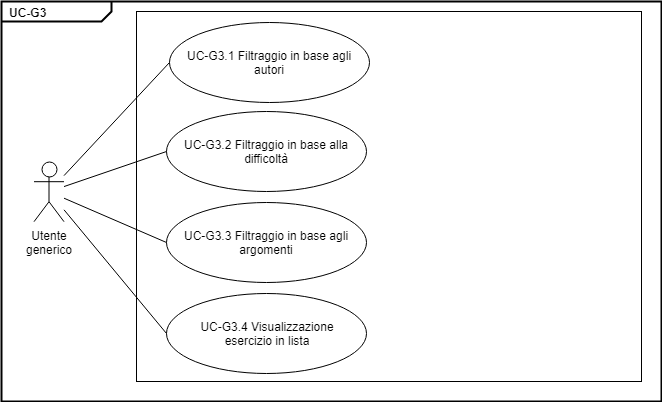
\includegraphics[scale=0.7]{images/UC-G3.png}
			\caption{UC-G3 Filtraggio esercizi}
		\end{figure}	

\subsubsection{UC-G3.1 Filtraggio in base agli autori}
	\begin{itemize}
		\item \textbf{Attori:} Utente generico.
		\item \textbf{Precondizione: } L'utente si trova nella vista di ricerca degli esercizi dell'applicazione.
		\item \textbf{Postcondizione: } L'utente ha indicato gli autori nel filtro di ricerca.
		\item \textbf{Scenario principale:}
		\begin{enumerate}
			\item l'utente visualizza la lista degli autori
			\item l'utente seleziona gli autori di cui vuole vedere gli esercizi
		\end{enumerate}
	\end{itemize}

\subsubsection{UC-G3.2 Filtraggio in base alla difficoltà}
	\begin{itemize}
		\item \textbf{Attori:} Utente generico.
		\item \textbf{Precondizione: } L'utente si trova nella vista di ricerca degli esercizi dell'applicazione.
		\item \textbf{Postcondizione: } L'utente ha indicato la difficoltà nel filtro di ricerca.
		\item \textbf{Scenario principale:}
		\begin{enumerate}
			\item l'utente visualizza i livelli possibili di difficoltà (da 1 a 5)
			\item l'utente indica il livello di difficoltà degli esercizi cercati
		\end{enumerate}
	\end{itemize}

	\subsubsection{UC-G3.3 Filtraggio in base agli argomenti}
		\begin{itemize}
			\item \textbf{Attori:} Utente generico.
			\item \textbf{Precondizione: } L'utente si trova nella vista di ricerca degli esercizi dell'applicazione.
			\item \textbf{Postcondizione: } L'utente ha indicato gli autori nel filtro di ricerca.
			\item \textbf{Scenario principale:}
			\begin{enumerate}
				\item l'utente visualizza la lista degli argomenti (pronomi, verbi, aggettivi, articoli, avverbi, ecc..)
				\item l'utente seleziona gli argomenti di cui vuole vedere gli esercizi
			\end{enumerate}
		\end{itemize}
		
\subsubsection{UC-G3.4 Visualizzazione esercizio in lista}
		\begin{itemize}
			\item \textbf{Attori:} Utente generico.
			\item \textbf{Precondizione: } L'utente si trova nella vista di ricerca degli esercizi dell'applicazione.
			\item \textbf{Postcondizione: } L'utente visualizza le informazioni di un esercizio.
			\item \textbf{Scenario principale:}
			\begin{enumerate}
				\item l'utente visualizza la frase inserita come esercizio
				\item l'utente visualizza la data di inserimento dell'esercizio
			\end{enumerate}
		\end{itemize}

	\subsubsection{UC-G4 Svolgimento esercizio}
		\begin{itemize}
			\item \textbf{Attori:} Utente generico.
			\item \textbf{Precondizione:}  L'utente visualizza la vista per l'esecuzione dell'esercizio.
			\item \textbf{Postcondizione:} L'utente visualizza la valutazione dell'esercizio.
			\item \textbf{Scenario principale:}
				\begin{enumerate}
					\item l'utente compila i campi (UC-G4.1).
					\item l'utente conferma i dati inseriti.
					\item l'utente visualizza la valutazione.
				\end{enumerate}
		\end{itemize}

	\subsubsection{UC-G4.1 Compilazione dei campi}
		\begin{itemize}
			\item \textbf{Attori:} Utente generico.
			\item \textbf{Precondizione:} L'utente ha selezionato un esercizio da eseguire.
			\item \textbf{Postcondizione:} L'utente ha compilato i campi proposti dall'esercizio.
			\item \textbf{Scenario principale:}
				\begin{enumerate}
					\item l'utente sceglie la classe grammaticale per ogni parola presentata
					\item l'utente conferma la soluzione dell'esercizio
				\end{enumerate}
		\end{itemize}
		
%TODO: inclusione in immagine e codice UC
	\subsubsection{UC-G5 Visualizzazione della valutazione dell'esercizio}
	\begin{itemize}
			\item \textbf{Attori:} Utente generico.
			\item \textbf{Precondizione:} L'utente ha completato l'esecuzione dell'esercizio.
			\item \textbf{Postcondizione:} L'allievo visualizza la valutazione dell'esercizio.
			\item \textbf{Scenario principale:}
				\begin{enumerate}
					\item l'allievo seleziona il correttore dell'esercizio (insegnante o algoritmo automatico)
					\item l'allievo visualizza la valutazione (da 1 a 10) in base al correttore scelto
				\end{enumerate}
	\end{itemize}				

\subsubsection{UC-G6 Segnalazione abuso di un esercizio}
	\begin{itemize}
		\item \textbf{Attori:} Utente generico.
		\item \textbf{Precondizione:} L'utente si trova nella vista di svolgimento di un esercizio che ritiene non conforme alle norme di comportamento.
		\item \textbf{Postcondizione:} L'utente ha inviato una notifica di abuso del codice di comportamento.
		\item \textbf{Scenario principale:}
		\begin{enumerate}
			\item l'utente seleziona l'opzione "Segnala abuso"
		\end{enumerate}
	\end{itemize}
	
	

\subsection{Elenco dei casi d'uso - Utente: Utente non riconosciuto}

\subsubsection{UC-N1 Visualizzazione pagina di registrazione}
	\begin{itemize}
		\item \textbf{Attori:} Utente non riconosciuto.
		\item \textbf{Precondizione:} L'utente si trova nella vista principale dell'applicazione.
		\item \textbf{Postcondizione:} L'utente si trova nella vista di registrazione dell'applicazione.
		\item \textbf{Scenario principale:}
		\begin{enumerate}
			\item l'utente seleziona l'opzione "Registrati"
		\end{enumerate}
	\end{itemize}


\subsubsection{UC-N2 Registrazione utente}
\begin{itemize}
		\item \textbf{Attori: }Utente non riconosciuto.
		\item \textbf{Precondizione: }L'utente si trova nella vista di registrazione dell'applicazione.
		\item \textbf{Postcondizione: }L'utente è registrato nel database locale.
		\item \textbf{Scenario principale: }
		\begin{enumerate}
		\item l'utente ha scelto di registrarsi al sistema, quindi di creare un nuovo profilo
		\item l'utente inserisce il proprio nome (UC-N2.1)
		\item l'utente inserisce il proprio cognome (UC-N2.2)
		\item l'utente inserisce l'username (UC-N2.3)
		\item l'utente inserisce la propria email (UC-N2.4)
		\item l'utente inserisce la password (UC-N2.5)
		\item l'utente fornirà il nome della scuola a cui appartiene (UC-N2.6)
		\item l'utente fornirà la città in cui si trova la scuola (UC-N2.7)
		\item l'utente indica il ruolo
		\item l'utente conferma la registrazione
		\end{enumerate}
		\item \textbf{Estensioni: }
		\begin{itemize}
			\item 10.a Nel caso in cui l'utente tenti l'inserimento di campi non validi vedrà comparire un messaggio d'errore "Campi non validi" (UC-N5).
		\end{itemize}
\end{itemize}

\begin{figure}[h]
	\centering
	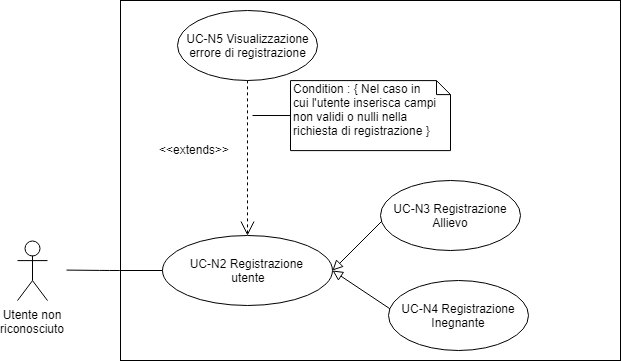
\includegraphics[scale=0.7]{images/UC-N2.png}
	\caption{UC-N2 Registrazione utente}
\end{figure}

\subsubsection{UC-N2.1 Inserimento nome: registrazione}
\begin{itemize}
	\item \textbf{Attori: }Utente non riconosciuto.
	\item \textbf{Precondizione: }L'utente si trova nella vista 		di registrazione dell'applicazione.
	\item \textbf{Postcondizione: }L'utente ha inserito il nome durante la procedura di registrazione.
	\item \textbf{Scenario principale: }
	\begin{enumerate}
		\item l'utente inserisce il proprio nome nella cella 				dedicata
	\end{enumerate}
\end{itemize}

\subsubsection{UC-N2.2 Inserimento cognome: registrazione}
\begin{itemize}
	\item \textbf{Attori: }Utente non riconosciuto.
	\item \textbf{Precondizione: }L'utente si trova nella vista 		di registrazione dell'applicazione.
	\item \textbf{Postcondizione: }L'utente ha inserito il cognome durante la procedura di registrazione.
	\item \textbf{Scenario principale: }
	\begin{enumerate}
		\item l'utente inserisce il proprio cognome nella cella 				dedicata
	\end{enumerate}
\end{itemize}

\subsubsection{UC-N2.3 Inserimento username: registrazione}
\begin{itemize}
	\item \textbf{Attori: }Utente non riconosciuto.
	\item \textbf{Precondizione: }L'utente si trova nella vista 		di registrazione dell'applicazione.
	\item \textbf{Postcondizione: }L'utente ha inserito l'username durante la procedura di registrazione.
	\item \textbf{Scenario principale: }
	\begin{enumerate}
		\item l'utente inserisce il proprio username nella cella dedicata
	\end{enumerate}
\end{itemize}

\subsubsection{UC-N2.4 Inserimento email: registrazione}
\begin{itemize}
	\item \textbf{Attori: }Utente non riconosciuto.
	\item \textbf{Precondizione: }L'utente si trova nella vista 		di registrazione dell'applicazione.
	\item \textbf{Postcondizione: }L'utente ha inserito l'email durante la procedura di registrazione.
	\item \textbf{Scenario principale: }
	\begin{enumerate}
		\item l'utente inserisce la propria email nella cella dedicata
	\end{enumerate}
\end{itemize}

\subsubsection{UC-N2.5 Inserimento password: registrazione}
\begin{itemize}
	\item \textbf{Attori: }Utente non riconosciuto.
	\item \textbf{Precondizione: }L'utente si trova nella vista 		di registrazione dell'applicazione.
	\item \textbf{Postcondizione: }L'utente ha inserito la password durante la procedura di registrazione.
	\item \textbf{Scenario principale: }
	\begin{enumerate}
		\item l'utente inserisce la password nella cella dedicata
	\end{enumerate}
\end{itemize}

\subsubsection{UC-N2.6 Inserimento nome scuola: registrazione}
\begin{itemize}
	\item \textbf{Attori: }Utente non riconosciuto.
	\item \textbf{Precondizione: }L'utente si trova nella vista 		di registrazione dell'applicazione.
	\item \textbf{Postcondizione: }L'utente ha inserito il nome della scuola che frequenta durante la procedura di registrazione.
	\item \textbf{Scenario principale: }
	\begin{enumerate}
		\item l'utente inserisce il nome della scuola che frequenta nella cella dedicata
	\end{enumerate}
\end{itemize}

\subsubsection{UC-N2.7 Inserimento città: registrazione}
\begin{itemize}
	\item \textbf{Attori: }Utente non riconosciuto.
	\item \textbf{Precondizione: }L'utente si trova nella vista 		di registrazione dell'applicazione.
	\item \textbf{Postcondizione: }L'utente ha inserito la città a cui la scuola appartiene durante la procedura di registrazione.
	\item \textbf{Scenario principale: }
	\begin{enumerate}
		\item l'utente inserisce la città della scuola nella cella dedicata
	\end{enumerate}
\end{itemize}

\begin{figure}[htbp]
	\centering
	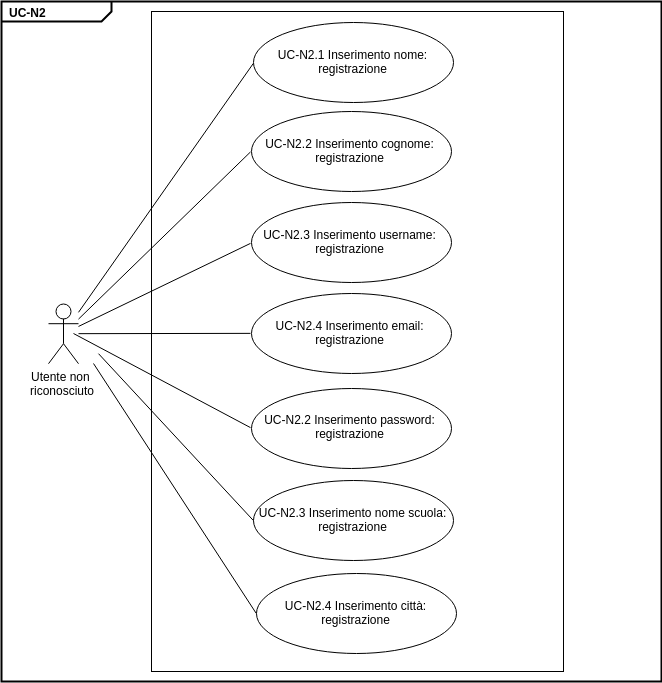
\includegraphics[scale=0.7]{images/UC-N2sub.png}
	\caption{Sottocasi di UC-N2}
\end{figure}


\subsubsection{UC-N3 Registrazione Allievo}
\begin{itemize}
	\item \textbf{Attori: }Utente non riconosciuto.
	\item \textbf{Precondizione: }L'utente si trova nella vista di registrazione dell'applicazione.
	\item \textbf{Postcondizione: }L'utente è registrato nel database locale come allievo.
	\item \textbf{Scenario principale: }
		\begin{enumerate}
		\item l'utente ha scelto di registrarsi al sistema, quindi di creare un nuovo profilo
		\item l'utente inserisce il proprio nome (UC-N2.1)
		\item l'utente inserisce il proprio cognome (UC-1.2)
		\item l'utente inserisce l'username (UC-N2.3)
		\item l'utente inserisce la propria email (UC-N2.4)
		\item l'utente inserisce la password (UC-N2.5)
		\item l'utente fornirà il nome della scuola a cui appartiene (UC-N2.6)
		\item l'utente fornirà la città in cui si trova la scuola (UC-N2.7)
		\item l'utente indica come ruolo "Allievo"
		\item l'utente conferma la registrazione
		\end{enumerate}
\end{itemize}

\subsubsection{UC-N4 Registrazione Insegnante}
\begin{itemize}
	\item \textbf{Attori: }Utente non riconosciuto.
	\item \textbf{Precondizione: }L'utente si trova nella vista di registrazione dell'applicazione.
	\item \textbf{Postcondizione: }L'utente è registrato nel database locale ed in attesa di conferma.
	\item \textbf{Scenario principale: }
		\begin{enumerate}
		\item l'utente ha scelto di registrarsi al sistema, quindi di creare un nuovo profilo
		\item l'utente inserisce il proprio nome (UC-N2.1)
		\item l'utente inserisce il proprio cognome (UC-N2.2)
		\item l'utente inserisce l'username (UC-N2.3)
		\item l'utente inserisce la propria email (UC-N2.4)
		\item l'utente inserisce la password (UC-N2.5)
		\item l'utente fornirà il nome della scuola a cui appartiene (UC-N2.6)
		\item l'utente fornirà la città in cui si trova la scuola (UC-N2.7)
		\item l'utente indica come ruolo "Insegnante"
		\item l'utente inserisce il proprio codice INPS (UC-N4.1)
		\item l'utente conferma la registrazione
		\end{enumerate}
\end{itemize}

\subsubsection{UC-N4.1 Inserimento codice INPS}
\begin{itemize}
	\item \textbf{Attori: }Utente non riconosciuto.
	\item \textbf{Precondizione: }L'utente si trova nella vista di registrazione dell'applicazione e ha indicato l'iscrizione come insegnante.
	\item \textbf{Postcondizione: }
		L'utente ha inserito il codice INPS durante la procedura di registrazione come insegnante.
		\item \textbf{Scenario principale:}
		\begin{enumerate}
			\item l'utente inserisce il codice INPS nella cella dedicata
		\end{enumerate}
\end{itemize}

\subsubsection{UC-N5 Visualizzazione errore di registrazione}
\begin{itemize}
	\item \textbf{Attori:} Utente non riconosciuto.
	\item \textbf{Precondizione:} L'utente ha confermato la richiesta di registrazione con campi non validi o nulli
	\item \textbf{Postcondizione:} L'utente torna alla vista di registrazione
	\item  \textbf{Scenario principale: }
	\begin{enumerate}
		\item visualizza un messaggio di errore "Registrazione non avvenuta: campi non validi"
	\end{enumerate}
\end{itemize}

\subsubsection{UC-N6 Autenticazione}
		\begin{itemize}
			\item \textbf{Attori:} Utente non riconosciuto.
			\item \textbf{Precondizione:} L'utente si trova nella vista di autenticazione dell'applicazione.
			\item \textbf{Postcondizione:} L'utente ha eseguito l'accesso con il proprio ruolo.
			\item \textbf{Scenario principale:}
				\begin{enumerate}
					\item l'utente inserisce il proprio username (UC-N6.1)
					\item l'utente inserisce la propria password (UC-N6.2)
					\item l'utente conferma l'accesso
				\end{enumerate}
				\item \textbf{Estensioni:}
				\begin{itemize}
					\item 2.a Nel caso in cui l'utente tenti l'inserimento di campi non validi vedrà comparire un messaggio d'errore (UC-N7).
				\end{itemize}
		\end{itemize}
		\begin{figure}[htbp]
			\centering
			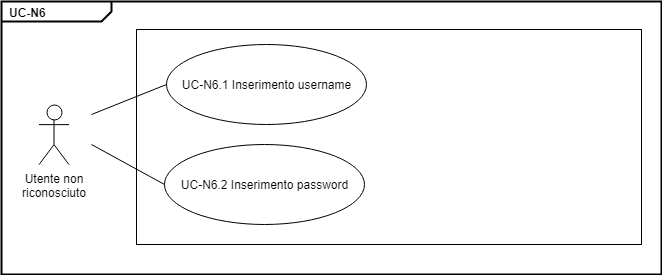
\includegraphics[scale=0.7]{images/UC-N6.png}
			\caption{UC-N6 Autenticazione}
		\end{figure}		
		
		

\subsubsection{UC-N6.1 Inserimento username: autenticazione}
\begin{itemize}
	\item \textbf{Attori:} Utente non riconosciuto.
			\item \textbf{Precondizione:} L'utente si trova nella vista di autenticazione dell'applicazione.
			\item \textbf{Postcondizione:} L'utente ha inserito il proprio username nella vista di autenticazione.
			\item \textbf{Scenario principale:}
				\begin{enumerate}
					\item l'utente scrive il proprio username nella cella apposita
				\end{enumerate}
\end{itemize}

\subsubsection{UC-N6.2 Inserimento password: autenticazione}
\begin{itemize}
	\item \textbf{Attori:} Utente non riconosciuto.
			\item \textbf{Precondizione:} L'utente si trova nella vista di autenticazione dell'applicazione.
			\item \textbf{Postcondizione:} L'utente ha inserito la propria password nella vista di autenticazione.
			\item \textbf{Scenario principale:}
				\begin{enumerate}
					\item l'utente scrive la propria password nella cella apposita
				\end{enumerate}
\end{itemize}
		
\subsubsection{UC-N7 Visualizzazione errore di autenticazione}
		\begin{itemize}
			\item \textbf{Attori:} Utente non riconosciuto.
			\item \textbf{Precondizione:} L'utente ha provato ad autenticarsi.
			\item \textbf{Postcondizione:} L'utente torna alla vista di accesso alla piattaforma.
			\item \textbf{Scenario principale:}
			\begin{enumerate}
				\item l'utente visualizza un messaggio di errore "Impossibile effettuare l'accesso: username o password errati"
			\end{enumerate}
		\end{itemize}
		
\subsection{Elenco dei casi d'uso - Utente: utente riconosciuto}
\subsubsection{UC-R1 Visualizzazione profilo personale}
\begin{itemize}
	\item \textbf{Attori:} Utente riconosciuto.
	\item \textbf{Precondizione:} L'utente si trova nella vista principale dell'applicazione.
	\item \textbf{Postcondizione:} L'utente si trova nella vista del proprio profilo.
	\item \textbf{Scenario principale:}
		\begin{enumerate}
			\item l'utente seleziona la voce "Profilo personale"
		\end{enumerate}
\end{itemize}

\subsubsection{UC-R2 Modifica profilo}
		\begin{itemize}
			\item \textbf{Attori:} Utente riconosciuto.
			\item \textbf{Precondizione:} L'utente si trova nella vista di modifica dei dati del proprio profilo.
			\item \textbf{Postcondizione:} L'utente ha modificato i propri dati personali.
			\item \textbf{Scenario principale:}
				\begin{enumerate}
					\item l'utente modifica l'username (UC-R2.1)
					\item  l'utente modifica la password (UC-R2.2)
					\item l'utente modifica la scuola che frequenta (UC-R2.3) 
					\item l'utente modifica la città a cui la scuola appartiene (UC-R2.4)
					\item l'utente conferma la modifica
				\end{enumerate}
				\item \textbf{Estensioni:}
				\begin{itemize}
					\item 2.a Nel caso in cui l'utente tenti l'inserimento di campi non validi vedrà comparire un messaggio d'errore (UC-R3).
				\end{itemize}
		\end{itemize}
		\begin{figure}[htbp]
			\centering
			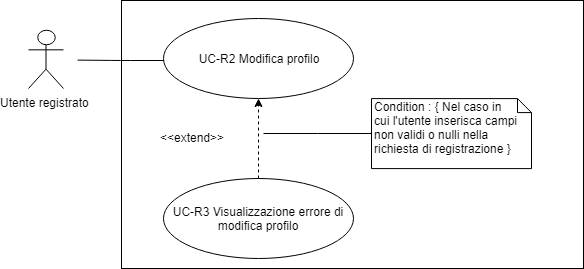
\includegraphics[scale=0.7]{images/UC-R2.png}
			\caption{UC-R2 Modifica profilo}
		\end{figure}
				\begin{figure}[htbp]
			\centering
			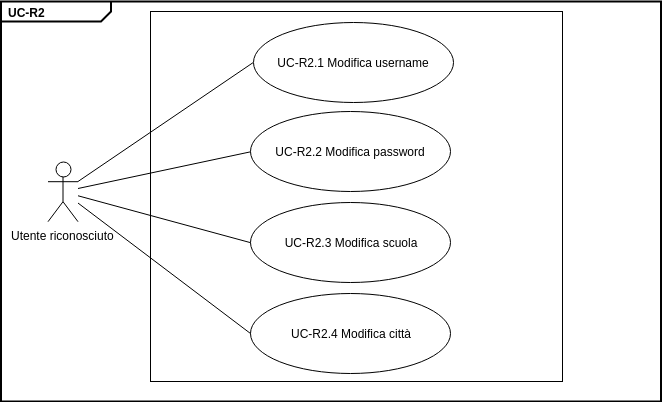
\includegraphics[scale=0.7]{images/UC-R2sub.png}
			\caption{Sottocasi di UC-R2}
		\end{figure}
		
\subsubsection{UC-R2.1 Modifica username}
\begin{itemize}
			\item \textbf{Attori:} Utente riconosciuto.
			\item \textbf{Precondizione:} L'utente si trova nella vista di modifica dei dati del proprio profilo.
			\item \textbf{Postcondizione:} L'utente ha modificato il proprio username.
			\item \textbf{Scenario principale:}
			\begin{enumerate}
				\item l'utente inserisce il nuovo username nella cella apposita
			\end{enumerate}
\end{itemize}

\subsubsection{UC-R2.2 Modifica password}
\begin{itemize}
			\item \textbf{Attori:} Utente riconosciuto.
			\item \textbf{Precondizione:} L'utente si trova nella vista di modifica dei dati del proprio profilo.
			\item \textbf{Postcondizione:} L'utente ha modificato la propria password.
			\item \textbf{Scenario principale:}
			\begin{enumerate}
				\item l'utente inserisce la nuova password nella cella apposita
			\end{enumerate}
\end{itemize}

\subsubsection{UC-R2.3 Modifica scuola}
\begin{itemize}
			\item \textbf{Attori:} Utente riconosciuto.
			\item \textbf{Precondizione:} L'utente si trova nella vista di modifica dei dati del proprio profilo.
			\item \textbf{Postcondizione:} L'utente ha modificato la scuola a cui appartiene.
			\item \textbf{Scenario principale:}
			\begin{enumerate}
				\item l'utente inserisce la scuola a cui appartiene nella cella apposita
			\end{enumerate}
\end{itemize}

\subsubsection{UC-R2.4 Modifica città}
\begin{itemize}
			\item \textbf{Attori:} Utente riconosciuto.
			\item \textbf{Precondizione:} L'utente si trova nella vista di modifica dei dati del proprio profilo.
			\item \textbf{Postcondizione:} L'utente ha modificato la città a cui la scuola appartiene.
			\item \textbf{Scenario principale:}
			\begin{enumerate}
				\item l'utente inserisce la città a cui la scuola appartiene nella cella apposita
			\end{enumerate}
\end{itemize}

\subsubsection{UC-R3 Visualizzazione errore di modifica del profilo}	
	\begin{itemize}
		\item \textbf{Attori:} Utente riconosciuto.
		\item \textbf{Precondizione:} L'utente ha inserito dei campi non validi o nulli nella modifica del proprio profilo.
		\item \textbf{Postcondizione:} L'utente torna alla vista del proprio profilo.
		\item \textbf{Scenario principale:}
		\begin{enumerate}
			\item l'utente visualizza un messaggio di errore "Modifica del profilo non avvenuta: campi non validi o nulli"
		\end{enumerate}
	\end{itemize}

\subsubsection{UC-R4 Logout}
\begin{itemize}
		\item \textbf{Attori:} Utente riconosciuto.
		\item \textbf{Precondizione:} L'utente si trova in una qualsiasi vista dell'applicazione.
		\item \textbf{Postcondizione:} L'utente si è disconnesso dalla piattaforma.
		\item \textbf{Scenario principale:}
		\begin{enumerate}
			\item l'utente seleziona l'opzione "Logout"
		\end{enumerate}
	\end{itemize}

\subsection{Elenco dei casi d'uso - Utente: moderatore}	
\subsubsection{UC-M1 Verifica richiesta insegnante}
		\begin{itemize}
			\item \textbf{Attori:} Moderatore.
			\item \textbf{Precondizione:} Il moderatore si trova nella vista di amministrazione dell'applicazione.
			\item \textbf{Postcondizione:} Il moderatore ha confermato o rifiutato l'utente richiedente il ruolo di insegnante.
			\item \textbf{Scenario principale:}
				\begin{enumerate}
					\item il moderatore visualizza la lista contenente l'username degli utenti che richiedono il ruolo di insegnante (UC-M1.1)
					\item il moderatore seleziona un utente dalla lista
					\item il moderatore decide l'esito della richiesta
				\end{enumerate}
		\end{itemize}	
		
\subsubsection{UC-M1.1 Visualizzazione lista richiedenti ruolo insegnante}
	\begin{itemize}
		\item \textbf{Attori:} Moderatore.
		\item \textbf{Precondizione:} Il moderatore si trova nella vista di amministrazione dell'applicazione.
		\item \textbf{Postcondizione:} Il moderatore visualizza la lista di coloro che hanno fatto richiesta di registrazione come insegnante.
		\item \textbf{Scenario principale:}
			\begin{enumerate}
				\item il moderatore visualizza gli utenti che hanno fatto richiesta del ruolo insegnante (UC-M1.1.1)
			\end{enumerate}
	\end{itemize}
		
\subsubsection{UC-M1.1.1 Visualizzazione utenti richiedenti ruolo di insegnante}
	\begin{itemize}
		\item \textbf{Attori:} Moderatore.
		\item \textbf{Precondizione:} Il moderatore si trova nella vista di amministrazione dell'applicazione.
		\item \textbf{Postcondizione:} Il moderatore visualizza le credenziali di un richiedente del ruolo di insegnante.
		\item \textbf{Scenario principale:}
			\begin{enumerate}
				\item il moderatore visualizza nome del richiedente
				\item il moderatore visualizza cognome del richiedente
				\item il moderatore visualizza il codice INPS del richiedente
			\end{enumerate}
	\end{itemize}			

\subsubsection{UC-M2 Visualizzazione lista degli esercizi: moderatore}
	\begin{itemize}
		\item \textbf{Attori:} Moderatore.
		\item \textbf{Precondizione:} Il moderatore ha eseguito l'accesso all'area Esercizi e può aver svolto una ricerca tra gli esercizi.
		\item \textbf{Postcondizione:} Il moderatore visualizza una lista di esercizi inseriti nella piattaforma.
		\item \textbf{Scenario principale:}
			\begin{enumerate}
				\item il moderatore visualizza gli esercizi all'interno di una lista (UC-M2.1)
			\end{enumerate}
	\end{itemize}
		
\subsubsection{UC-M2.1 Visualizzazione esercizio inserito}
	\begin{itemize}
		\item \textbf{Attori:} Moderatore.
		\item \textbf{Precondizione:} Il moderatore ha eseguito l'accesso all'area Esercizi e può aver svolto una ricerca tra gli esercizi.
		\item \textbf{Postcondizione:} Il moderatore visualizza le informazioni di un esercizio presente nella piattaforma.
		\item \textbf{Scenario principale:}
			\begin{enumerate}
				\item il moderatore visualizza il codice associato all'esercizio
				\item il moderatore visualizza la frase dell'esercizio
				\item il moderatore visualizza l'username dell'autore dell'esercizio
				\item il moderatore visualizza la data in cui l'esercizio è stato inserito
			\end{enumerate}
	\end{itemize}		
		
\subsubsection{UC-M3 Ricerca esercizi: moderatore}
	\begin{itemize}
		\item \textbf{Attori:} Moderatore.
		\item \textbf{Precondizione:} Il moderatore ha effettuato l'accesso nell'area esercizi.
		\item \textbf{Postcondizione:} Il moderatore ottiene una lista degli esercizi contenenti la parola o le parole ricercate.
		\item \textbf{Scenario principale:}
			\begin{enumerate}
				\item il moderatore scrive nella barra di ricerca una frase o una sua parte
			\end{enumerate}
	\end{itemize}
	
\subsubsection{UC-M4 Eliminazione di un esercizio}
			\begin{itemize}
			\item \textbf{Attori:} Moderatore.
			\item \textbf{Precondizione:} Il moderatore visualizza la lista di esercizi.
			\item \textbf{Postcondizione:} Il moderatore ha eliminato l'esercizio desiderato.
			\item \textbf{Scenario principale:}
				\begin{enumerate}
					\item il moderatore indica gli esercizi da eliminare
					\item il moderatore conferma l'eliminazione dell'esercizio selezionato
				\end{enumerate}
		\end{itemize}

\subsubsection{UC-M5 Visualizzazione lista degli utenti: moderatore}
	\begin{itemize}
		\item \textbf{Attori:} Moderatore.
		\item \textbf{Precondizione:} Il moderatore ha eseguito l'accesso all'area Utenti e può aver svolto una ricerca tra gli utenti.
		\item \textbf{Postcondizione:} Il moderatore visualizza la lista degli utenti presenti nella piattaforma.
		\item \textbf{Scenario principale:}
			\begin{enumerate}
				\item il moderatore visualizza gli utenti presenti nella piattaforma (UC-M5.1)
			\end{enumerate}
	\end{itemize}
	
\subsubsection{UC-M5.1 Visualizzazione utente iscritto in lista}
	\begin{itemize}
		\item \textbf{Attori:} Moderatore.
		\item \textbf{Precondizione:} Il moderatore ha eseguito l'accesso all'area Utenti e può aver svolto una ricerca tra gli utenti.
		\item \textbf{Postcondizione:} Il moderatore visualizza le credenziali di un utente iscritto alla piattaforma.
		\item \textbf{Scenario principale:}
			\begin{enumerate}
				\item il moderatore visualizza il nome dell'utente
				\item il moderatore visualizza il cognome dell'utente
				\item il moderatore visualizza l'username di un utente
			\end{enumerate}
	\end{itemize}
		
\subsubsection{UC-M6 Ricerca utenti: moderatore}
	\begin{itemize}
		\item \textbf{Attori:} Moderatore.
		\item \textbf{Precondizione:} Il moderatore visualizza la lista degli utenti presenti nella piattaforma.
		\item \textbf{Postcondizione:} Il moderatore ottiene una lista degli utenti aventi nell'username la parola indicata.
		\item \textbf{Scenario principale:}
			\begin{enumerate}
				\item il moderatore scrive nella barra di ricerca una stringa
				\item il moderatore visualizza una lista di utenti il cui username contiene la stringa ricercata
			\end{enumerate}
	\end{itemize}
	
\subsubsection{UC-M7 Eliminazione di un utente}
\begin{itemize}
	\item \textbf{Attori:} Moderatore.
	\item \textbf{Precondizione:} Il moderatore visualizza la lista degli utenti.
	\item \textbf{Postcondizione:} Il moderatore ha eliminato l'utente desiderato.
	\item \textbf{Scenario principale:}
	\begin{enumerate}
		\item il moderatore indica uno o più utenti da eliminare
		\item il moderatore conferma l'eliminazione degli utenti selezionati
	\end{enumerate}
\end{itemize}

\subsubsection{UC-M8 Visualizzazione lista delle segnalazioni}
\begin{itemize}
	\item \textbf{Attori:} Moderatore.
	\item \textbf{Precondizione:} Il moderatore si trova nella vista di amministrazione dell'applicazione.
	\item \textbf{Postcondizione:} Il moderatore visualizza la lista delle segnalazioni ricevute.
	\item \textbf{Scenario principale:}
	\begin{enumerate}
		\item il moderatore seleziona l'opzione "Lista delle segnalazioni"
		\item il moderatore visualizza le segnalazioni effettuate (UC-M8.1)
	\end{enumerate}
\end{itemize}

\subsubsection{UC-M8.1 Visualizzazione segnalazione in lista}
\begin{itemize}
	\item \textbf{Attori:} Moderatore.
	\item \textbf{Precondizione:} Il moderatore si trova nella vista di amministrazione dell'applicazione.
	\item \textbf{Postcondizione:} Il moderatore visualizza le specifiche di una segnalazione.
	\item \textbf{Scenario principale:}
	\begin{enumerate}
		\item il moderatore visualizza la frase segnalata
		\item il moderatore visualizza la data della segnalazione
		\item il moderatore visualizza l'username dell'autore dell'esercizio segnalato
		\item il moderatore visualizza l'username dell'autore della segnalazione
	\end{enumerate}
\end{itemize}

\subsubsection{UC-M9 Eliminazione segnalazione}
\begin{itemize}
	\item \textbf{Attori:} Moderatore.
	\item \textbf{Precondizione:} Il moderatore visualizza la lista delle segnalazioni ricevute.
	\item \textbf{Postcondizione:} Il moderatore ha eliminato la segnalazione desiderata.
	\item \textbf{Scenario principale:}
	\begin{enumerate}
		\item Il moderatore seleziona la segnalazione
		\item Il moderatore seleziona l'opzione "Elimina segnalazione"
	\end{enumerate}
\end{itemize}

\subsubsection{UC-M10 Accesso all'area Esercizi}
\begin{itemize}
	\item \textbf{Attori:} Moderatore.
	\item \textbf{Precondizione:} Il moderatore si trova nell'area di amministrazione dell'applicazione.
	\item \textbf{Postcondizione:} Il moderatore ha eseguito l'accesso all'area esercizi.
	\item \textbf{Scenario principale:}
	\begin{enumerate}
		\item il moderatore seleziona l'opzione "Area esercizi"
	\end{enumerate}
\end{itemize}

\subsubsection{UC-M11 Accesso all'area Utenti}
\begin{itemize}
	\item \textbf{Attori:} Moderatore.
	\item \textbf{Precondizione:} Il moderatore si trova nell'area di amministrazione dell'applicazione.
	\item \textbf{Postcondizione:} Il moderatore ha eseguito l'accesso all'area utenti.
	\item \textbf{Scenario principale:}
	\begin{enumerate}
		\item il moderatore seleziona l'opzione "Area utenti"
	\end{enumerate}
\end{itemize}

\subsection{Elenco dei casi d'uso - Utente: insegnante}		
\subsubsection{UC-I1 Visualizzazione lista esercizi inseriti}
\begin{itemize}
\item \textbf{Attori: }Insegnante.
		\item \textbf{Precondizione: }L'insegnante si trova nell'area Esercizi inseriti e può aver svolto una ricerca tra gli esercizi.
		\item \textbf{Postcondizione: }L'insegnante visualizza una lista di esercizi inseriti. 
		\item \textbf{Scenario principale:}
		\begin{enumerate}
			\item l'insegnante visualizza gli esercizi inseriti (UC-I1.1)
		\end{enumerate}
	\end{itemize}

\subsubsection{UC-I1.1 Visualizzazione esercizio inserito trovato}
\begin{itemize}
\item \textbf{Attori: }Insegnante.
		\item \textbf{Precondizione: }L'insegnante si trova nell'area Esercizi inseriti e può aver svolto una ricerca tra gli esercizi.
		\item \textbf{Postcondizione: }L'insegnante visualizza le specifiche di un esercizio inserito. 
		\item \textbf{Scenario principale:}
		\begin{enumerate}
			\item l'insegnante visualizza la frase dell'esercizio
			\item l'insegnante visualizza la data di inserimento dell'esercizio
		\end{enumerate}
	\end{itemize}

\subsubsection{UC-I2 Ricerca esercizi inseriti}
\begin{itemize}
	\item \textbf{Attori:} Insegnante.
	\item \textbf{Precondizione:} L'insegnante ha effettuato l'accesso all'area esercizi inseriti.
	\item \textbf{Postcondizione:} L'insegnante ottiene la lista degli esercizi contenenti la parola o le parole cercate.
	\item \textbf{Scenario principale:}
		\begin{enumerate}
				\item l'insegnante scrive nella barra di ricerca una frase o una sua parte
		\end{enumerate}
\end{itemize}

\subsubsection{UC-I3 Modifica soluzione}
\begin{itemize}
	\item \textbf{Attori:} Insegnante.
	\item \textbf{Precondizione:} L'insegnante visualizza la lista degli esercizi inseriti.
	\item \textbf{Postcondizione:} La soluzione inserita è stata modificata.
	\item \textbf{Scenario principale:}
		\begin{enumerate}
		\item l'insegnante visualizza le parole della frase associate alle classi grammaticali indicati nella precedente soluzione
		\item l'insegnante modifica le classi grammaticali associate alle parole dell'esercizio
		\item l'insegnante conferma la modifica
		\end{enumerate}
\end{itemize}
	
\subsubsection{UC-I4 Eliminare una soluzione di un esercizio}
\begin{itemize}
	\item \textbf{Attori:} Insegnante.
	\item \textbf{Precondizione:} L'insegnante visualizza la lista degli esercizi inseriti.
	\item \textbf{Postcondizione:} Le soluzioni selezionate vengono eliminate.
	\item \textbf{Scenario principale:}
		\begin{enumerate}
			\item l'insegnante seleziona una o più soluzioni da eliminare
			\item l'insegnante conferma l'eliminazione
		\end{enumerate}
\end{itemize}

\subsubsection{UC-I5 Visualizzazione area di inserimento nuovo esercizio}
\begin{itemize}
		\item \textbf{Attori: }Insegnante.
		\item \textbf{Precondizione: }L'insegnante è nella vista principale dell'applicazione.
		\item \textbf{Postcondizione: }L'insegnante è nella vista di inserimento di un nuovo esercizio.
		\item \textbf{Scenario principale: }
	\begin{enumerate} 
		\item l'insegnante seleziona la voce "Inserisci esercizio"
	\end{enumerate}
\end{itemize}

\subsubsection{UC-I6 Inserimento esercizio}
	\begin{itemize}
		\item \textbf{Attori: }Insegnante.
		\item \textbf{Precondizione: }L'insegnante è nella vista di inserimento di un nuovo esercizio.
		\item \textbf{Postcondizione: }L'esercizio è stato inserito.
		\item \textbf{Scenario principale: }
			\begin{enumerate} 
				\item l'insegnante inserisce la frase
				\item l'insegnante inserisce la soluzione (UC-I6.1)
				\item l'insegnante inserisce gli argomenti (UC-I6.2)
				\item l'insegnante inserisce la difficoltà (UC-I6.3)
				\item l'insegnante conferma l'inserimento
			\end{enumerate}
		\item \textbf{Estensioni:} 
			\begin{itemize}
				\item 1.a Nel caso in cui la frase inserita sia nulla, viene visualizzato un errore (UC-I7)
			\end{itemize}
	\end{itemize}
	
	\begin{figure}[h]
		\centering
		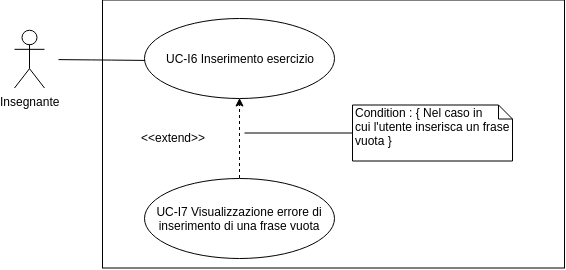
\includegraphics[scale=0.7]{images/UC-I6ext.png}
		\caption{UC-I6 Inserimento esercizio}
	\end{figure}
	\begin{figure}[h]
		\centering
		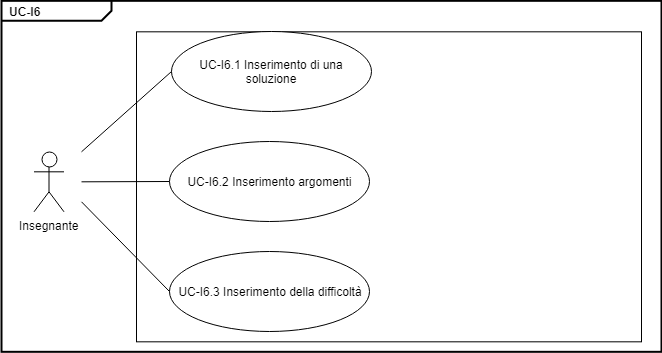
\includegraphics[scale=0.7]{images/UC-I6.png}
		\caption{Sottocasi di UC-I6}
	\end{figure}

\subsubsection{UC-I6.1 Inserimento di una soluzione}
\begin{itemize}
\item \textbf{Attori: }Insegnante.
\item \textbf{Precondizione: }L'insegnante è nella vista di inserimento di un nuovo esercizio.
\item \textbf{Postcondizione: }L'insegnante ha inserito la propria soluzione.
\item \textbf{Scenario principale: }
		\begin{enumerate} 
		\item l'insegnante visualizza la soluzione proposta dal generatore automatico
		\item l'insegnante può modificare le classi grammaticali assegnate dal generatore automatico che ritiene errate
		\item l'insegnante seleziona lo stato della soluzione inserita, pubblica o privata
		\item l'insegnante conferma la soluzione
		\end{enumerate}	
\end{itemize}

\subsubsection{UC-I6.2 Inserimento argomenti}
\begin{itemize}
\item \textbf{Attori: }Insegnante.

\item \textbf{Precondizione:} L'insegnante sta inserendo un esercizio, gli viene richiesta la compilazione di una lista di argomenti presenti nell'esercizio.
\item \textbf{Postcondizione:} L'insegnante ha selezionato gli argomenti trattati nell'esercizio.
\item \textbf{Scenario principale: }
		\begin{enumerate}
		\item l'insegnante visualizza la lista degli argomenti
		\item l'insegnante seleziona gli argomenti che vengono toccati nell'esercizio
		\end{enumerate}
\end{itemize}				

\subsubsection{UC-I6.3 Inserimento della difficoltà}
\begin{itemize}
	\item \textbf{Attori: }Insegnante.
	\item \textbf{Precondizione:} L'insegnante è nella vista di inserimento di un nuovo esercizio.
	\item \textbf{Postcondizione:} L'insegnante ha indicato il livello di difficoltà.
	\item \textbf{Scenario principale:}
	\begin{enumerate}
		\item l'insegnante visualizza i livelli possibili di difficoltà (da 1 a 5)
		\item l'insegnante indica il livello di difficoltà dell'esercizio da inserire
	\end{enumerate}
\end{itemize}

\subsubsection{UC-I7 Visualizzazione errore di inserimento di una frase vuota}
\begin{itemize}
	\item \textbf{Attori:} Insegnante.
	\item \textbf{Precondizione:} L'insegnante è nella vista di inserimento di un nuovo esercizio e ha inserito una frase vuota.
	\item \textbf{Postcondizione:} L'insegnante torna alla vista di inserimento dell'esercizio.
	\item \textbf{Scenario principale:}
	\begin{enumerate}
		\item l'insegnante visualizza un messaggio di errore "La frase inserita è vuota"
	\end{enumerate}
\end{itemize}

\subsubsection{UC-I8 Creazione di una classe}
\begin{itemize}
	\item \textbf{Attori:} Insegnante.
	\item \textbf{Precondizione:} L'insegnante si trova nella vista del proprio profilo.
	\item \textbf{Postcondizione:} L'insegnante si trova nella vista di gestione della classe creata.
	\item \textbf{Scenario principale:}
	\begin{enumerate}
		\item l'insegnante selezione l'opzione "Crea classe"
		\item l'insegnante inserisce il nome della classe (UC-I8.1)
		\item l'insegnante inserisce la descrizione della classe (UC-I8.2)
		\item l'insegnante conferma la creazione
	\end{enumerate}
\end{itemize}

\begin{figure}[h]
		\centering
		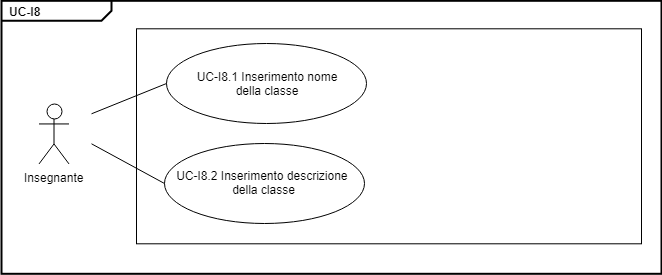
\includegraphics[scale=0.7]{images/UC-I8.png}
		\caption{UC-I8 Creazione di una classe}
	\end{figure}

\subsubsection{UC-I8.1 Inserimento nome della classe}
\begin{itemize}
	\item \textbf{Attori:} Insegnante.
	\item \textbf{Precondizione:} L'insegnante si trova nella vista del proprio profilo e ha selezionato la creazione di una nuova classe.
	\item \textbf{Postcondizione:} L'insegnante ha inserito il nome della classe durante la creazione della classe.
	\item \textbf{Scenario principale:}
	\begin{enumerate}
		\item l'insegnante inserisce il nome della classe nella cella appropriata
	\end{enumerate}
\end{itemize}

\subsubsection{UC-I8.2 Inserimento desrizione della classe}
\begin{itemize}
	\item \textbf{Attori:} Insegnante.
	\item \textbf{Precondizione:} L'insegnante si trova nella vista del proprio profilo e ha selezionato la creazione di una nuova classe.
	\item \textbf{Postcondizione:} L'insegnante ha inserito la descrizione della classe durante la creazione della classe.
	\item \textbf{Scenario principale:}
	\begin{enumerate}
		\item l'insegnante inserisce la descrizione della classe nella cella appropriata
	\end{enumerate}
\end{itemize}

\subsubsection{UC-I9 Eliminazione di una classe}
\begin{itemize}
	\item \textbf{Attori:} Insegnante.
	\item \textbf{Precondizione:} L'insegnante si trova nella vista di gestione di una propria classe.
	\item \textbf{Postcondizione:} L'insegnante elimina la classe dal sistema.
	\item \textbf{Scenario principale:}
	\begin{enumerate}
		\item l'insegnante clicca sul pulsante di eliminazione della classe
		\item l'insegnante conferma l'eliminazione
	\end{enumerate}
\end{itemize}

\subsubsection{UC-I10 Inserimento alunni}
\begin{itemize}
	\item \textbf{Attori:} Insegnante.
	\item \textbf{Precondizione:} L'insegnante si trova nella vista di gestione di una propria classe.
	\item \textbf{Postcondizione:} L'insegnante visualizza gli alunni inseriti.
	\item \textbf{Scenario principale:}
	\begin{enumerate}
		\item l'insegnante seleziona l'opzione "Aggiungi alunni"
		\item l'insegnante indica gli studenti da aggiungere (UC-I10.1)
		\item l'insegnante conferma l'inserimento
	\end{enumerate}
\end{itemize}

\subsubsection{UC-I10.1 Selezione alunni per l'inserimento}
\begin{itemize}
	\item \textbf{Attori:} Insegnante.
	\item \textbf{Precondizione:} l'insegnante si trova nella vista di aggiunta degli alunni a una classe
	\item \textbf{Postcondizione:} l'insegnante ha indicato gli alunni da inserire nella classe
	\item \textbf{Scenario principale:}
	\begin{enumerate}
		\item l'insegnante visualizza la lista di tutti gli alunni presenti sulla piattaforma
		\item l'insegnante ricerca gli alunni da inserire
		\item l'insegnante seleziona gli alunni da inserire
	\end{enumerate}
\end{itemize}

\subsubsection{UC-I11 Assegnazione esercizi}
\begin{itemize}
	\item \textbf{Attori:} Insegnante.
	\item \textbf{Precondizione:} Visualizza una lista di esercizi da una ricerca eseguita.
	\item \textbf{Postcondizione:} L'insegnante ha assegnato esercizi alla classe.
	\item \textbf{Scenario principale:}
	\begin{enumerate}
		\item l'insegnante seleziona degli esercizi in lista da assegnare
		\item l'insegnante indica la classe a cui assegnarli
		\item l'insegnante conferma l'assegnazione
	\end{enumerate}
\end{itemize}

\subsubsection{UC-I12 Visualizzazione lista delle classi}		
\begin{itemize}
	\item \textbf{Attori:} Insegnante.
	\item \textbf{Precondizione:} L'insegnante si trova nella vista del proprio profilo.
	\item \textbf{Postcondizione:} L'insegnante visualizza la lista delle classi create.
	\item \textbf{Scenario principale:}
	\begin{enumerate}
		\item l'insegnante seleziona l'opzione "vedi classi"
		\item l'insegnante visualizza le classi create (UC-I12.1)
	\end{enumerate}		
\end{itemize}

\subsubsection{UC-I12.1 Visualizzazione classe in lista}		
\begin{itemize}
	\item \textbf{Attori:} Insegnante.
	\item \textbf{Precondizione:} L'insegnante si trova nella vista del proprio profilo.
	\item \textbf{Postcondizione:} L'insegnante visualizza le informazioni riguardanti una classe.
	\item \textbf{Scenario principale:}
	\begin{enumerate}
		\item l'insegnante visualizza il nome della classe creata
		\item l'insegnante visualizza la descrizione della classe creata
		\item l'insegnante visualizza la data di creazione della classe
		\item l'insegnante visualizza il numero di alunni iscritti alla classe
	\end{enumerate}		
\end{itemize}

\subsubsection{UC-I13 Visualizzazione area di gestione di una classe}
\begin{itemize}
	\item \textbf{Attori:} Insegnante.
	\item \textbf{Precondizione:} L'insegnante visualizza la lista delle classi create.
	\item \textbf{Postcondizione:} L'insegnante visualizza la vista di gestione di una propria classe.
	\item \textbf{Scenario principale:}
	\begin{enumerate}
		\item l'insegnante seleziona una classe
	\end{enumerate}
\end{itemize}

\subsubsection{UC-I14 Visualizzazione lista degli alunni iscritti alla classe}		
\begin{itemize}
	\item \textbf{Attori:} Insegnante.
	\item \textbf{Precondizione:} L'insegnante si trova nella vista di gestione di una propria classe.
	\item \textbf{Postcondizione:} L'insegnante visualizza l'elenco degli alunni iscritti.
	\item \textbf{Scenario principale:}
	\begin{enumerate}
		\item l'insegnante seleziona l'opzione "vedi alunni"
		\item l'insegnante visualizza gli alunni iscritti alla classe (UC-I14.1)
			\end{enumerate}		
\end{itemize}

\subsubsection{UC-I14.1 Visualizzazione alunno iscritto alla classe in lista}		
\begin{itemize}
	\item \textbf{Attori:} Insegnante.
	\item \textbf{Precondizione:} L'insegnante si trova nella vista di gestione di una propria classe.
	\item \textbf{Postcondizione:} L'insegnante visualizza le credenziali di un alunno iscritto alla classe.
	\item \textbf{Scenario principale:}
	\begin{enumerate}
		\item l'insegnante visualizza il nome dell'alunno iscritto alla classe
		\item l'insegnante visualizza il cognome dell'alunno iscritto alla classe
		\item l'insegnante visualizza l'username dell'alunno iscritto alla classe
			\end{enumerate}		
\end{itemize}

\subsubsection{UC-I15 Visualizzare i progressi di un alunno della classe}
\begin{itemize}
	\item \textbf{Attori:} Insegnante.
	\item \textbf{Precondizione}: L'insegnante visualizza la lista degli alunni iscritti alla classe.
	\item \textbf{Postcondizione:} L'insegnante visualizza i progressi relativi allo studente selezionato.
	\item \textbf{Scenario principale:}
	\begin{enumerate}
		\item l'insegnante seleziona uno studente
		\item l'insegnante visualizza i grafici che riportano la media totale, la media per tipologia di esercizi e lo sviluppo della media nel tempo
	\end{enumerate}
\end{itemize}

\subsubsection{UC-I16 Elimina alunno dalla classe}		
\begin{itemize}
	\item \textbf{Attori:} Insegnante.
	\item \textbf{Precondizione:} L'insegnante visualizza la lista degli alunni della classe.
	\item \textbf{Postcondizione:} L'insegnante ha rimosso l'allievo dalla classe.
	\item \textbf{Scenario principale:}
	\begin{enumerate}
		\item l'insegnante seleziona l'allievo da rimuovere dalla classe
		\item l'insegnante conferma l'eliminazione
	\end{enumerate}	
\end{itemize}

\subsubsection{UC-I17 Accesso all'area Esercizi inseriti}		
\begin{itemize}
	\item \textbf{Attori:} Insegnante.
	\item \textbf{Precondizione:} L'insegnante si trova nell'area del proprio profilo personale.
	\item \textbf{Postcondizione:} L'insegnante ha eseguito l'accesso all'area esercizi inseriti.
	\item \textbf{Scenario principale:}
	\begin{enumerate}
		\item l'insegnante seleziona l'opzione "Area esercizi inseriti"
	\end{enumerate}	
\end{itemize}

\subsubsection{UC-I18 Visualizzazione lista alunni da aggiungere alla classe}
\begin{itemize}
	\item \textbf{Attori:} Insegnante.
	\item \textbf{Precondizione:} l'insegnante si trova nella vista di aggiunta degli alunni a una classe
	\item \textbf{Postcondizione:} l'insegnante visualizza la lista di tutti gli alunni presenti sulla piattaforma.
	\item \textbf{Scenario principale:}
	\begin{enumerate}
		\item l'insegnante visualizza gli alunni iscritti alla piattaforma (UC-I18.1)
	\end{enumerate}
\end{itemize}

\subsubsection{UC-I18.1 Visualizzazione alunno da aggiungere alla classe}
\begin{itemize}
	\item \textbf{Attori:} Insegnante.
	\item \textbf{Precondizione:} l'insegnante si trova nella vista di aggiunta degli alunni a una classe
	\item \textbf{Precondizione:} l'insegnante visualizza le credenziali di un alunno da aggiungere in una classe.
	\item \textbf{Scenario principale:}
	\begin{enumerate}
		\item l'insegnante visualizza il nome dell'alunno
		\item l'insegnante visualizza il cognome dell'alunno
		\item l'insegnante visualizza l'username dell'alunno
	\end{enumerate}
\end{itemize}

\subsubsection{UC-I19 Ricerca alunno}
\begin{itemize}
	\item \textbf{Attori:} Insegnante.
	\item \textbf{Precondizione:} L'insegnante visualizza la lista di tutti gli alunni presenti sulla piattaforma.
	\item \textbf{Postcondizione:} L'insegnante visualizza una lista di username contenenti la stringa inserita.
	\item \textbf{Scenario principale:}
	\begin{enumerate}
		\item l'insegnante scrive l'username di un alunno, o una sua parte
	\end{enumerate}
\end{itemize}

\subsection{Elenco dei casi d'uso - Utente: allievo}
	\subsubsection{UC-A1 Visualizzazione progressi}
	\begin{itemize}
			\item \textbf{Attori:} Allievo.
			\item \textbf{Precondizione:} L'allievo si trova nella vista del proprio profilo.
			\item \textbf{Postcondizione:} L'allievo visualizza i progressi svolti fino a quel momento.
			\item \textbf{Scenario principale:}
				\begin{enumerate}
					\item L'allievo visualizza la media delle valutazioni ricevute, la media per tipologia di esercizi e lo sviluppo della media nel tempo
				\end{enumerate}
	\end{itemize}
	
	\subsubsection{UC-A2 Visualizzazione lista delle classi di appartenenza}
		\begin{itemize}
			\item \textbf{Attori:} Allievo.
			\item \textbf{Precondizione:} L'allievo si trova nella vista del proprio profilo.
			\item \textbf{Postcondizione:} L'allievo visualizza la lista delle classi a cui appartiene.
			\item \textbf{Scenario principale:}
			\begin{enumerate}
				\item l'allievo seleziona l'opzione "Lista delle classi"
				\item l'allievo visualizza le classi a cui appartiene
			\end{enumerate}
		\end{itemize}			

\subsubsection{UC-A2.1 Visualizzazione classe di appartenenza in lista}
		\begin{itemize}
			\item \textbf{Attori:} Allievo.
			\item \textbf{Precondizione:} L'allievo si trova nella vista del proprio profilo.
			\item \textbf{Postcondizione:} L'allievo visualizza le informazioni di una classe a cui appartiene.
			\item \textbf{Scenario principale:}
			\begin{enumerate}
				\item L'allievo visualizza il nome della classe
				\item L'allievo visualizza il nome dell'insegnante creatore della classe
				\item L'allievo visualizza il cognome dell'insegnante creatore della classe
				\item L'allievo visualizza la descrizione della classe
			\end{enumerate}
		\end{itemize}	

	\subsubsection{UC-A3 Annullamento dell'iscrizione a una classe}
		\begin{itemize}
			\item \textbf{Attori:} Allievo.
			\item \textbf{Precondizione:} L'allievo visualizza la lista delle classi a cui appartiene.
			\item \textbf{Postcondizione:} L'allievo ha annullato l'iscrizione alla classe.
			\item \textbf{Scenario principale:}
			\begin{enumerate}
				\item l'allievo seleziona l'opzione "Disiscriviti" in corrispondenza di una classe
			\end{enumerate}
		\end{itemize}					
				
	\subsubsection{UC-A4 Visualizzazione delle informazioni della classe}
		\begin{itemize}
			\item \textbf{Attori:} Allievo.
			\item \textbf{Precondizione:} L'allievo visualizza la lista delle classi a cui appartiene.
			\item \textbf{Postcondizione:} L'allievo visualizza le informazioni della classe indicata (allievi iscritti, media delle valutazioni ed esercizi assegnati).
			\item \textbf{Scenario principale:}
			\begin{enumerate}
				\item l'allievo seleziona una classe
			\end{enumerate}
		\end{itemize}
		
\subsubsection{UC-A5 Seleziona esercizio assegnato}
\begin{itemize}
			\item \textbf{Attori:} Allievo.
			\item \textbf{Precondizione:} L'allievo visualizza le informazioni della classe indicata (allievi iscritti, media delle valutazioni ed esercizi assegnati).
			\item \textbf{Postcondizione:} L'allievo visualizza la vista per l'esecuzione dell'esercizio.
			\item \textbf{Scenario principale:}
			\begin{enumerate}
				\item l'allievo seleziona un esercizio assegnato
			\end{enumerate}
		\end{itemize}

		\subsubsection{UC-15 Ricerca dei dati delle annotazioni}
		\begin{figure}[h]
			\centering
			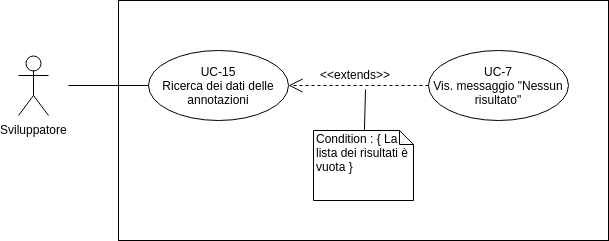
\includegraphics[scale=0.7]{images/UC-15.png}
			\caption{UC-15 Ricerca dei dati delle annotazioni}
		\end{figure}			
	
		\begin{itemize}
			\item Attori: Sviluppatore
			\item Precondizione: Lo sviluppatore si trova nella vista principale dell'applicazione
			\item Postcondizione: Lo sviluppatore ottiene una lista delle annotazioni correnti delle frasi
			\item Scenario principale:
				\begin{enumerate}
					\item lo sviluppatore accede all'area dei dati;
					\item lo sviluppatore scrive nella barra di ricerca una sottostringa della frase cercata (possibilmente nulla);
					\item (UC-15.1) lo sviluppatore seleziona i filtri da usare nella ricerca (possibilmente nessuno).
				\end{enumerate}
			\item Estensioni:
				\begin{itemize}
					\item 3.a Se non viene trovato un risultato, viene visualizzato un messaggio di avviso (UC-7)
				\end{itemize}
		\end{itemize}


	
	\subsubsection{UC-15.1 Filtraggio dei dati}	
		\begin{figure}[h]
			\centering
			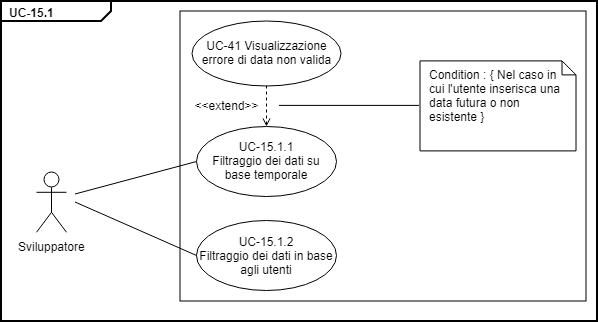
\includegraphics[scale=0.7]{images/UC-15_1.png}
			\caption{UC-15.1 Filtraggio dei dati}
		\end{figure}	
		\begin{itemize}
			\item Attori: Sviluppatore
			\item Precondizione: Lo sviluppatore si trova nell'area dati e ha scritto nella barra di ricerca una sottostringa della frase cercata
			\item Postcondizione: Lo sviluppatore ottiene una lista di frasi in base al filtro selezionato
			\item Scenario principale:
				\begin{enumerate}
					\item lo sviluppatore seleziona il filtro su base temporale (UC-15.1.1);
					\item lo sviluppatore seleziona il filtro in base agli utenti (UC-15.1.2);
					\item lo sviluppatore indica dei parametri per restringere la ricerca;
					\item lo sviluppatore esegue la ricerca.
				\end{enumerate}	
			\item Estensioni:
				\begin{itemize}
					\item 4.a Se i parametri inseriti dall'utente non sono coerenti viene mostrato un messaggio di errore (UC-5).
				\end{itemize}		
		\end{itemize}
	
	
	\subsubsection{UC-15.1.1 Filtraggio dei dati su base temporale}	
		\begin{figure}[h]
			\centering
			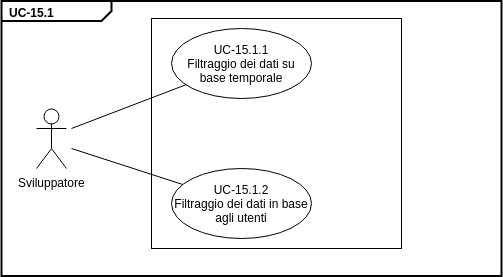
\includegraphics[scale=0.7]{images/UC-15_1_1.png}
			\caption{UC-15.1.1 Filtraggio dei dati su base temporale e UC-15.1.2 Filtraggio dei dati in base agli utenti}
		\end{figure}			
		\begin{itemize}
			\item Attori: Sviluppatore
			\item Precondizione: Lo sviluppatore si trova nell'area dati e ha scritto nella barra di ricerca una sottostringa della frase cercata.
			\item Postcondizione: Lo sviluppatore ottiene una lista di frasi in base al range temporale indicato.
			\item Scenario principale:
				\begin{enumerate}
					\item lo sviluppatore seleziona il filtro;
					\item lo sviluppatore indica due date che definiscono un intervallo di tempo per restringere la ricerca;
				\end{enumerate}
		\end{itemize}	
	
	\subsubsection{UC-15.1.2 Filtraggio dei dati in base agli utenti}	
		\begin{itemize}
			\item Attori: Sviluppatore
			\item Precondizione: Lo sviluppatore si trova nell'area dati e ha scritto nella barra di ricerca una sottostringa della frase cercata.
			\item Postcondizione: Lo sviluppatore ottiene una lista di frasi in base agli utenti scelti.
			\item Scenario principale:
				\begin{enumerate}
					\item lo sviluppatore seleziona il filtro (inclusione o esclusione di un utente);
					\item lo sviluppatore indica l'utente (o la lista di utenti);
					\item lo sviluppatore esegue la ricerca.
				\end{enumerate}
		\end{itemize}	
	\subsubsection{UC-16 Visualizzazione dei dati di una annotazione di una frase}
		\begin{itemize}
			\item Attori: Sviluppatore
			\item Precondizione: Lo sviluppatore si trova nell'area dati e ha a disposizione i risultati della ricerca delle annotazioni
			\item Postcondizione: Lo sviluppatore legge i dati di una annotazione di una frase
			\item Scenario principale:
				\begin{enumerate}
					\item lo sviluppatore sceglie una annotazione.
				\end{enumerate}
		\end{itemize}
	
	\subsubsection{UC-17 Visualizzazione storico}
		\begin{figure}[h]
			\centering
			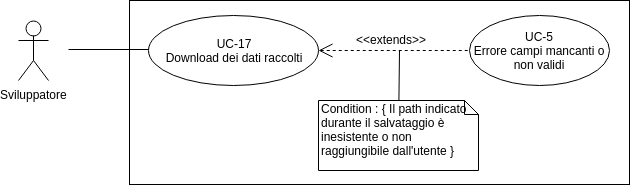
\includegraphics[scale=0.7]{images/UC-17.png}
			\caption{UC-17 Visualizzazione storico}
		\end{figure}	
		\begin{itemize}
			\item Attori: Sviluppatore
			\item Precondizione: Lo sviluppatore si trova nell'area dati e ha a disposizione i risultati della ricerca delle annotazioni.
			\item Postcondizione: Lo sviluppatore ottiene lo storico delle annotazioni ottenuta nella ricerca precedente.
			\item Scenario principale:
			\begin{enumerate}
				\item lo sviluppatore seleziona l'opzione "vedi storico"
			\end{enumerate}
		\end{itemize}
		
	\subsubsection{UC-18 Ordinamento dei risultati}
		\begin{itemize}
			\item Attori: Sviluppatore
			\item Precondizione: Lo sviluppatore si trova nell'area dati con i risultati della ricerca effettuata.
			\item Postcondizione: Lo sviluppatore ottiene la lista precedente ordinata in base alle scelte effettuate.
			\item Scenario principale:
				\begin{enumerate}
					\item lo sviluppatore sceglie il parametro secondo il quale ordinare i risultati (frase, frequenza, ultima correzione, utente);
					\item lo sviluppatore richiede l'ordinamento scelto.
				\end{enumerate}
		\end{itemize} 
	
	\subsubsection{UC-19 Download dei dati raccolti}
		\begin{itemize}
			\item Attori: Sviluppatore
			\item Precondizione: Lo sviluppatore si trova nell'area dati con i risultati della ricerca effettuata.
			\item Postcondizione: Lo sviluppatore ottiene un file con i dati dei risultati precedentemente trovati.
			\item Scenario principale:
				\begin{enumerate}
					\item lo sviluppatore richiede il download dei dati;
					\item lo sviluppatore decide il path in cui il file viene salvato;
					\item lo sviluppatore esegue il salvataggio.
				\end{enumerate}
			\item Estensioni:
				\begin{itemize}
					\item 2.a se il path indicato è inesistente, viene visualizzato un messaggio di errore (UC-5).
				\end{itemize}
		\end{itemize} 

	% Cosa si intende esattamente con modello?
		
	\subsubsection{UC-20 Visualizzazione di un modello}
		\begin{itemize}
			\item Attori: Sviluppatore
			\item Precondizione: Lo sviluppatore si trova nella vista principale dell'applicazione.
			\item Postcondizione: Lo sviluppatore ottiene le informazioni di un modello.
			\item Scenario principale:
			\begin{enumerate}
				\item lo sviluppatore accede all'area modelli;
				\item lo sviluppatore seleziona un modello.
			\end{enumerate}
	\end{itemize}
	
	\subsubsection{UC-21 Download di un modello}
		\begin{figure}[h]
			\centering
			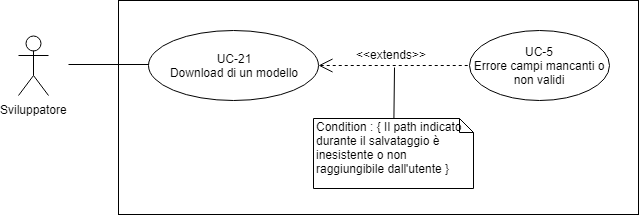
\includegraphics[scale=0.7]{images/UC-21.png}
			\caption{UC-21 Download di un modello}
		\end{figure}			
		\begin{itemize}
			\item Attori: Sviluppatore
			\item Precondizione: Lo sviluppatore si trova nella vista con le informazioni del modello selezionato.
			\item Postcondizione: Lo sviluppatore ottiene un file con il modello.
			\item Scenario principale:
			\begin{enumerate}
					\item lo sviluppatore richiede il download del modello;
					\item lo sviluppatore decide il path in cui il file viene salvato;
					\item lo sviluppatore esegue il salvataggio.
				\end{enumerate}
			\item Estensioni:
				\begin{itemize}
					\item 2.a se il path indicato è inesistente, viene visualizzato un messaggio di errore (UC-5).
				\end{itemize}
		\end{itemize}
		
	\subsubsection{UC-22 Creazione di un modello}
		\begin{figure}[h]
			\centering
			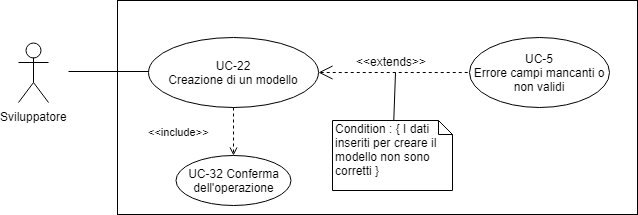
\includegraphics[scale=0.7]{images/UC-22.png}
				\caption{UC-22 Creazione di un modello}
		\end{figure}			
		\begin{itemize}
			\item Attori: Sviluppatore
			\item Precondizione: Lo sviluppatore si trova nella vista principale dell'applicazione.
			\item Postcondizione: Lo sviluppatore aggiunge un modello alla piattaforma.
			\item Scenario principale:
			\begin{enumerate}
				\item lo sviluppatore accede all'area modelli;
				\item lo sviluppatore seleziona la funzione di aggiunta di un modello;
				\item lo sviluppatore inserisce i dati per la creazione del modello;
				\item lo sviluppatore completa la creazione.
			\end{enumerate}
			\item Estensioni:
				\begin{itemize}
					\item 4.a se uno dei dati inseriti non è coerente, allora viene visualizzato un messaggio di errore (UC-5).
				\end{itemize}
		\end{itemize}
	\subsubsection{UC-23 Eliminazione di un esercizio}
			\begin{itemize}
			\item Attori: amministratore;
			\item Precondizione: l'amministratore si trova nella vista di amministrazione dell'applicazione;
			\item Postcondizione: l'amministratore ha eliminato l'esercizio desiderato.
			\item Scenario principale:
				\begin{enumerate}
					\item l'amministratore indica l'esercizio da eliminare;
					\item l'amministratore conferma l'eliminazione dell'esercizio selezionato.
				\end{enumerate}
		\end{itemize}
		\newpage	
	\section{Requisiti}
		In questa sezione viene assegnato un codice ad ogni requisito al fine di facilitarne l'identificazione. L'assegnazione avverrà secondo le condizioni stabilite dal gruppo nel documento \textit{NormeDiProgetto\_v3.0.0}, riportate in seguito. 
\subsection{Denominazione dei requisiti}
Si vuole associare un identificatore univoco per ogni requisito individuato durante l'analisi dei requisiti. Si \`e deciso di utilizzare il seguente formato:
  \begin{center}
    R[Priorità][Tipo][Codice]
	\end{center}
dove:
	\begin{itemize}
	\item il campo “\textbf{Priorità}” può assumere uno dei seguenti 	valori:
		\begin{itemize}
  		\item \textbf{O}: indica un requisito obbligatorio, irrinunciabile per il committente;
		\item \textbf{D}: indica un requisito desiderabile ma non strettamente necessario;
		\item \textbf{P}: indica un requisito opzionale, che potrebbe venir soddisfatto o meno senza che il prodotto risulti mancante di funzionalità essenziali.
		\end{itemize}
	\item il campo “\textbf{Tipo}” può assumere uno dei seguenti valori:
		\begin{itemize}
  		\item \textbf{F}: definisce un requisito funzionale, ovvero un requisito che indica quale deve essere la reazione del software in specifici casi (ad esempio con  un determinato input);
		\item \textbf{Q}: definisce un requisito di qualità$^*$, ovvero un requisito votato a garantire efficienza, efficacia e qualità al prodotto;
		\item \textbf{V}: definisce un requisito di vincolo, ovvero un requisito imposto dalla proponente del capitolato;
		\item \textbf{R}: definisce un requisito prestazionale, ovvero un requisito relativo alle prestazioni di sistema.
		\end{itemize}
	\item il campo “\textbf{Codice}” assumerà un valore numerico intero positivo, univoco ed incrementale.
	\end{itemize}
\newpage
\subsection{Requisiti funzionali}
\begin{tabularx}{\textwidth}{| c | p{10cm} | X |}
		\rowcolor{LightBlue}
		\color{white}\bfseries Requisito & \color{white}\bfseries Descrizione & \color{white}\bfseries Fonti\\[0.25cm]
		ROF1 & L'utente può aggiungere una frase da svolgere come esercizio. & UC-G1 \newline Interno\\
		ROF2 & L'utente deve poter selezionare un esercizio da svolgere tra quelli ricercati nella piattaforma. & UC-G2 \newline Interno\\
		ROF3 & L'utente deve poter ricercare degli esercizi sulla piattaforma. & UC-G3\newline Capitolato\\
		RPF1 & Durante la ricerca, l'utente può impostare il filtro secondo gli autori. & UC-G3.1 \newline Interno\\
		RPF2 & Durante la ricerca, l'utente può impostare il filtro secondo la difficoltà. & UC-G3.2 \newline Interno\\
		RPF3 & Durante la ricerca, l'utente può impostare il filtro secondo gli argomenti trattati. & UC-G3.3 \newline Interno\\
		RPF4 & L'utente deve visualizzare frase e data di inserimento dell'esercizio in lista. & UC-G3.4 \newline Interno\\
		ROF4 & L'utente deve poter svolgere un esercizio da lui indicato. & UC-G4 \newline Capitolato\\
		ROF5 & L'utente deve poter inserire una frase da svolgere o selezionare un esercizio da quelli disponibili sul sistema. & UC-G4.1 \newline Capitolato\\
		ROF6 & L'utente deve visualizzare la valutazione dell'esercizio da lui svolto. & UC-G5\newline Capitolato\\
		RPF5 & L'utente può segnalare un esercizio per abuso delle regole comportamentali. & UC-G6\newline Interno\\
		
		RDF1 & L'utente potrà accedere alla pagina di registrazione alla piattaforma. & UC-N1 \newline Interno\\
		ROF7 & L'utente non riconosciuto si registra alla piattaforma. & UC-N2\newline Interno\\
		ROF8 & L'utente non riconosciuto inserisce il proprio nome mentre si registra alla piattaforma. & UC-N2.1 \newline Interno\\
		ROF9 & L'utente non riconosciuto inserisce il proprio cognome mentre si registra alla piattaforma . & UC-N2.2 \newline Interno\\
		ROF10 & L'utente non riconosciuto inserisce l'username mentre si registra alla piattaforma. & UC-N2.3 \newline Interno\\
		ROF11 & L'utente non riconosciuto inserisce la propria email mentre si registra alla piattaforma. & UC-N2.4 \newline Interno\\
		ROF12 & L'utente non riconosciuto inserisce la password mentre si registra alla piattaforma. & UC-N2.5 \newline Interno\\
		ROF13 & L'utente non riconosciuto inserisce il nome della scuola che frequenta mentre si registra alla piattaforma. & UC-N2.6 \newline Interno\\
		ROF14 & L'utente non riconosciuto inserisce la città a cui la scuola appartiene mentre si registra alla piattaforma. & UC-N2.7 \newline Interno\\
		ROF15 & L'utente non riconosciuto si registra alla piattaforma come allievo. & UC-N3 \newline Interno\\			
		ROF16 & L'utente non riconosciuto si registra alla piattaforma come insegnante. & UC-N4 \newline Interno\\
		ROF17 & L'utente non riconosciuto inserisce il proprio codice INPS mentre si registra alla piattaforma come insegnante. & UC-N4.1 \newline Interno\\
		RDF2 & L'utente non riconosciuto viene avvisato in caso di errore nell'inserimento dei dati al momento della registrazione. & UC-N5 \newline Interno\\
		ROF18 & L'utente non riconosciuto esegue l'accesso alla piattaforma utilizzando le sue credenziali. & UC-N6 \newline Interno\\
		ROF19 & L'utente non riconosciuto inserisce il proprio username mentre esegue l'accesso alla piattaforma. & UC-N6.1 \newline Interno\\
		ROF20 & L'utente non riconosciuto inserisce la propria password mentre esegue l'accesso alla piattaforma. & UC-N6.2 \newline Interno\\
		ROF21 & L'utente non riconosciuto viene avvisato in caso di errore nell'inserimento dei dati al momento dell'autenticazione. & UC-N7 \newline Interno\\

		RDF3 & L'utente riconosciuto può accedere alla vista del proprio profilo personale. & UC-R1 \newline Interno\\
		RDF4 & L'utente riconosciuto modifica i dati del proprio profilo personale. & UC-R2 \newline Interno\\
		RDF5 & L'utente riconosciuto modifica il proprio username mentre modifica il profilo. & UC-R2.1 \newline Interno\\
		RDF6 & L'utente riconosciuto modifica la propria password mentre modifica il profilo. & UC-R2.2 \newline Interno\\
		RDF7 & L'utente riconosciuto modifica il nome della scuola che frequenta mentre modifica il profilo. & UC-R2.3 \newline Interno\\
		RDF8 & L'utente riconosciuto modifica la città a cui la scuola appartiene mentre modifica il profilo. & UC-R2.4 \newline Interno\\
		ROF22 & L'utente riconosciuto viene avvisato in caso di errore nella modifica delle proprie informazioni. & UC-R3 \newline Interno\\	
		RDF9 & L'utente riconosciuto può disconnettersi dalla piattaforma. & UC-R4 \newline Interno\\	
		
		RDF10 & Il moderatore verifica le credenziali di un utente che richiede la registrazione come insegnante. & UC-M1 \newline Interno\\
		RDF11 & Il moderatore visualizza una lista di utenti che richiedono la registrazione come insegnante. & UC-M1.1 \newline Interno\\
		RDF12 & Il moderatore visualizza le credenziali degli utenti che richiedono la registrazione come insegnante. & UC-M1.1.1 \newline Interno\\
		RDF13 & \textbf{DA ELIMINARE} & UC-M1.2 \newline Interno\\
		RDF14 & \textbf{DA ELIMINARE} & UC-M1.3 \newline Interno\\
		RDF15 & \textbf{DA ELIMINARE} & UC-M1.4 \newline Interno\\
		RDF16 & Il moderatore può visualizzare la lista degli esercizi inseriti nella piattaforma. & UC-M2 \newline Interno\\
		RDF17 & Il moderatore può visualizzare le informazioni riguardanti un esercizio inserito nella piattaforma. & UC-M2.1 \newline Interno\\
		RPF6 & Il moderatore può ricercare gli esercizi inserendo la frase o una parte di essa. & UC-M3 \newline Interno\\
		RPF7 & Il moderatore deve poter eliminare uno qualsiasi degli esercizi inseriti nel sistema. & UC-M4 \newline Interno\\
		RDF18 & Il moderatore può visualizzare la lista degli utenti iscritti alla piattaforma. & UC-M5 \newline Interno\\
		RDF19 & Il moderatore deve visualizzare nome e cognome e username dell'utente in lista. & UC-M5.1 \newline Interno\\
		RPF8 & Il moderatore può ricercare gli utenti inserendo l'username o una parte di esso. & UC-M6 \newline Interno\\
		RPF9 & Il moderatore può eliminare un utente iscritto alla piattaforma. & UC-M7 \newline Interno\\
		RPF10 & Il moderatore può visualizzare la lista delle segnalazioni effettuate dagli utenti. & UC-M8 \newline Interno\\
		RPF11 & Il moderatore deve visualizzare la frase, la data, l'autore dell'esercizio segnalato e l'autore della segnalazione in lista. & UC-M8.1 \newline Interno\\
		RPF12 & Il moderatore può eliminare una segnalazione dalla relativa lista. & UC-M9 \newline Interno\\
		RDF20 & Il moderatore deve poter accedere all'area esercizi. & UC-M10 \newline Interno\\
		RDF21 & Il moderatore deve poter accedere all'area utenti. & UC-M11 \newline Interno\\
		
		RDF22 & L'insegnante, accedendo alla sua area del profilo, può visualizzare la lista degli esercizi da lui creati. & UC-I1 \newline Interno\\
		RDF23 & L'insegnante, accedendo alla sua area del profilo, deve visualizzare la frase e la data di inserimento dell'esercizio inserito. & UC-I1.1 \newline Interno\\
		RDF24 & L'insegnante può ricercare gli esercizi che ha inserito inserendo la frase o una parte di essa. & UC-I2 \newline Interno\\
		RPF13 & L'insegnante può modificare una soluzione di un esercizio da lui fornita. & UC-I3 \newline Capitolato\\
		RPF14 & L'insegnante può eliminare una soluzione di un esercizio da lui fornita. & UC-I4 \newline Interno\\
		ROF23 & L'insegnante deve poter accedere all'area di inserimento nuovo esercizio. & UC-I5 \newline Interno\\		
		ROF24 & L'insegnante può inserire un esercizio nel sistema. & UC-I6 \newline Capitolato\\
		ROF25 & L'insegnante deve inserire la soluzione dell'esercizio che sta creando; può renderla pubblica o privata. & UC-I6.1 \newline Capitolato\\
		RPF15 & L'insegnante indica gli argomenti trattati nell'esercizio che sta creando. & UC-I6.2 \newline Interno\\
		RPF16 & L'insegnante indica il livello di difficoltà nell'esercizio che sta creando. & UC-I6.3 \newline Interno\\
		ROF26 & L'insegnante visualizzerà un messaggio di errore nel caso in cui stia inserendo una frase vuota come esercizio. & UC-I7 \newline Interno\\
		ROF27 & L'insegnante deve poter creare una nuova classe. & UC-I8 \newline Interno\\
		ROF28 & Durante la creazione di una classe, l'insegnante deve poter inserire un nome. & UC-I8.1 \newline Interno\\
		ROF29 & Durante la creazione di una classe, l'insegnante deve poter inserire una descrizione. & UC-I8.2 \newline Interno\\
		ROF30 & L'insegnante deve poter eliminare una classe dal sistema. & UC-I9 \newline Interno\\
		ROF31 & L'insegnante deve poter aggiungere degli alunni ad una classe. & UC-I10 \newline Interno\\
		RPF17 & L'insegnante deve indicare gli alunni da inserire nella classe. & UC-I10.1 \newline Interno\\
		RPF18 & Durante la ricerca degli alunni da inserire a una classe, l'insegnante deve visualizzare una lista contenente tutti gli alunni presenti sulla piattaforma. & UC-I10.1.1 \newline Interno\\
		RPF19 & Durante la ricerca degli alunni da inserire a una classe, l'insegnante deve visualizzare nome, cognome e username degli alunni in lista. & UC-I10.1.1.1 \newline Interno\\
		RPF20 & L'insegnante può ricercare un alunno da inserire nella classe tramite username. & UC-I10.1.2 \newline Interno\\
		ROF32 & L'insegnante deve poter aggiungere degli esercizi a quelli assegnati ad una classe. & UC-I11 \newline Interno\\
		ROF33 & L'insegnante deve poter visualizzare la lista delle proprie classi. & UC-I12 \newline Interno\\
		ROF34 & L'insegnante deve visualizzare il nome, la descrizione, la data di creazione e il numero di iscritti della classe in lista. & UC-I12.1 \newline Interno\\
		RDF25 & L'insegnante può visualizzare l'area per la gestione delle classi. & UC-I13 \newline Interno\\
		ROF35 & L'insegnante deve poter visualizzare la lista degli alunni iscritti ad una delle sue classi. & UC-I14 \newline Interno\\		
		ROF36 & L'insegnante deve visualizzare il nome, il cognome e l'username dell'alunno in lista iscritto alla classe. & UC-I14.1 \newline Interno\\
		RPF21 & L'insegnante potrebbe voler visualizzare i progressi degli alunni di una propria classe. & UC-I15 \newline Interno\\
		ROF37 & L'insegnante deve poter eliminare un alunno dalla lista di quelli iscritti ad una delle proprie classi. & UC-I16 \newline Interno\\
		RDF26 & L'insegnante deve poter accedere all'area del proprio profilo che riporta gli esercizi inseriti. & UC-I17 \newline Interno\\

		RDF27 & L'allievo, accedendo al proprio profilo, potrà visualizzare i dati relativi ai propri progressi. & UC-A1 \newline Capitolato\\		
		RDF28 & L'allievo può visualizzare la lista delle classi a cui appartiene. & UC-A2 \newline Interno\\
		RDF29 & L'allievo può visualizzare il nome e la descrizione della classe e il nome e il cognome dell'insegnante che ha creato la classe in lista. & UC-A2.1 \newline Interno\\
		RDF30 & L'allievo può annullare l'iscrizione ad una classe. & UC-A3 \newline Interno\\
		RDF31 & L'allievo può visualizzare le informazioni riguardanti una classe a cui appartiene e gli esercizi assegnati. & UC-A4 \newline Interno\\
		RPF22 & L'allievo può selezionare un esercizio assegnato. & UC-A5 \newline Interno\\

		RDF32 & Lo sviluppatore può ottenere una lista delle annotazioni di una particolare frase. & UC-S1 \newline Capitolato\\
		RDF33 & Lo sviluppatore deve poter filtrare i dati trovati durante la ricerca ottenendo una lista di annotazioni. & UC-S1.1 \newline Capitolato\\
		RDF34 & Lo sviluppatore deve visualizzare la data, l'username dell'autore dell'annotazione in lista e l'ID del relativo esercizio. & UC-S1.2 \newline Capitolato\\
		RDF35 & Lo sviluppatore può impostare un filtro temporale per la ricerca delle annotazioni. & UC-S1.1.1 \newline Interno\\
		RDF36 & Lo sviluppatore deve poter includere dalla ricerca di annotazioni solo uno o più utenti. & UC-S1.1.2 \newline Capitolato\\
		RDF37 & Lo sviluppatore durante l'inclusione di un utente deve poter cercare degli utenti & UC-S1.1.2.1 \newline Interno\\		
		RDF38 & Lo sviluppatore visualizzerà un messaggio di errore nel caso inserisca una data non valida durante il filtraggio di annotazioni in base temporale. & UC-S2 \newline Interno\\
		RPF23 & Lo sviluppatore deve poter visualizzare i dati relativi ad una particolare annotazione. & UC-S3 \newline Capitolato\\
		RPF24 & Lo sviluppatore deve poter visualizzare lo storico delle annotazioni. & UC-S4 \newline Capitolato\\
		RPF25 & Lo sviluppatore può ordinare la lista dei risultati ottenuti dalla ricerca tramite determinati parametri. & UC-S5 \newline Interno\\	
		ROF38 & Lo sviluppatore deve poter scaricare un file contenente i dati relativi agli esercizi ottenuti con la ricerca. & UC-S6 \newline Capitolato\\
		ROF39 & Lo sviluppatore deve poter scaricare un file contenente i dati relativi agli esercizi ottenuti con la ricerca in formato \texttt{.txt}. & UC-S7 \newline Capitolato\\
		RDF39 & Lo sviluppatore deve poter scaricare un file contenente i dati relativi agli esercizi ottenuti con la ricerca in formato \texttt{.csv}. & UC-S8 \newline Capitolato\\
		RDF40 & Lo sviluppatore deve poter scaricare un file contenente i dati relativi agli esercizi ottenuti con la ricerca in formato \texttt{.json}. & UC-S9 \newline Capitolato\\
		RDF41 & Lo sviluppatore visualizzerà un messaggio di errore nel caso in cui indichi un path non esistente al momento del download di file. & UC-S10 \newline Interno\\		
		RPF26 & Lo sviluppatore può visualizzare le informazioni relative ad un dataset. & UC-S11 \newline Interno\\
		RDF42 & Lo sviluppatore può visualizzare la lista dei modelli disponibili. & UC-S12 \newline Interno\\
		RDF43 & Lo sviluppatore deve visualizzare il nome e la lingua del modello in lista. & UC-S12.1 \newline Interno\\
		RPF27 & Lo sviluppatore deve poter scaricare un modello. & UC-S13 \newline Capitolato\\
		RPF28 & Lo sviluppatore può visualizzare informazioni riguardanti i modelli disponibili nella piattaforma. & UC-S14 \newline Interno\\
		RPF29 & Lo sviluppatore deve poter creare un modello tramite la piattaforma. & UC-S15 \newline Capitolato\\ 
		RDF44 & Lo sviluppatore visualizzerà un messaggio di errore se inserirà un dataset in un formato errato. & UC-S16 \newline Interno\\
		RPF30 & Lo sviluppatore può cambiare modello utilizzato dal software di apprendimento automatico. & UC-S17 \newline Interno\\
		
		\hline
		\caption{Tabella dei requisiti funzionali}
\end{tabularx}

\subsection{Requisiti di vincolo}
\begin{longtable}{| c | p{10cm} | c |}
		\rowcolor{LightBlue}
		\color{white}\bfseries Requisito & \color{white}\bfseries Descrizione & \color{white}\bfseries Fonti\\[0.25cm]
		ROV1 & Utilizzo del software di apprendimento automatico per il pos-tagging$^*$ Hunpos per lo svolgimento degli esercizi. & Capitolato \\
		RDV1 & Utilizzo di Google Firebase per l'immagazzinamento dei dati. & Capitolato \\
		RPV1 & Dovrebbe essere consentita la raccolta di dati in più lingue. & Capitolato \\
		ROV2 & L’interfaccia web deve essere sviluppata utilizzando HTML5, CSS3 e EcmaScript6 & Interno\\
		ROV3 & L'implementazione della gestione del database deve essere sviluppata utilizzando JavaScript(Node.js) & Interno\\
		ROV4 & La parte backend del software deve essere sviluppata utilizzando JavaScript (Node.js) & Interno\\
		\hline
		\caption{Tabella dei requisiti di vincolo}
\end{longtable}

\subsection{Requisiti di qualità}
\begin{longtable}{| c | p{10cm} | c |}
		\rowcolor{LightBlue}
		\color{white}\bfseries Requisito & \color{white}\bfseries Descrizione & \color{white}\bfseries Fonti\\[0.25cm]
		ROQ1 & Il gruppo deve fornire un'analisi dei requisiti come documentazione dell'applicazione alla proponente. & Capitolato \\
		ROQ2 & Il gruppo deve fornire una descrizione tecnica del prodotto alla proponente. & Capitolato \\ 
		RDQ1 & I commenti, i nomi delle funzioni e delle variabili del codice dovrebbero essere esplicativi ed in lingua inglese. & Capitolato \\ 
		RDQ2 & Il numero di parametri delle procedure deve essere al massimo 3. & Capitolato \\
		RPQ1 & La piattaforma deve essere fornita di un codice di comportamento per gli utenti & Interno\\
		RDQ3 & I documenti devono avere un indice di \textit{Gulpease} di almeno 50 & Interno\\
		ROQ3 & Tutte le norme stabilite nel documento \textit{NormeDiProgetto\_v3.0.0} devono essere rispettate & Interno\\
		RDQ4 & Il numero di linee di codice di ogni procedura non deve essere maggiore di 20. & Capitolato\\
		RDQ5 & Il valore della complessità ciclomatica$^*$ (stabilito nelle \textit{NormeDiProgetto\_v3.0.0}) deve essere minore di 10. & Capitolato\\
		\hline
		\caption{Tabella dei requisiti di qualità}
\end{longtable}
		\subsection{Tracciamento dei requisiti}
\begin{longtable}{| p{5cm} | p{5cm} |}
		\rowcolor{LightBlue}
		\color{white}\bfseries Fonte & \color{white}\bfseries Requisito \\[0.25cm]
		Interno & 	ROF1 \newline
					ROF2 \newline
					RDF1 \newline
					RDF2 \newline
					RDF3 \newline
					RPF1 \newline
					RDF4 \newline
					RDF5 \newline
					RPF2 \newline
					RPF4 \newline
					RPF5 \newline
					RPF6 \newline
					RPF7 \newline
					RDF9 \newline
					RPF10 \newline
					ROF10 \newline
					ROF11 \newline
					ROF12 \newline
					ROF13 \newline
					ROF14 \newline
					ROF15 \newline
					ROF16 \newline
					RPF13 \newline
					RDF11 \\
					
		\rowcolor{LightGray}
		Capitolato & 	ROF3 \newline
						RPF3\newline
						ROF4\newline
						ROF5\newline
						RDF6\newline
						ROF6\newline
						ROF7\newline
						ROF8\newline
						RDF7\newline
						RDF8\newline
						RDF10\newline
						RPF8\newline
						RPF9\newline
						ROF9\newline
						RPF11\newline
						RPF12\newline
						ROV1\newline
						RDV1\newline
						ROV2\newline
						RDV2\newline
						RPV1\newline
						ROQ1\newline
						ROQ2\newline
						RDQ1 \\
		
		
		
		UC-1 & ROF1 \\
		\rowcolor{LightGray}
		UC-2 & ROF2 \\
		UC-3 & RDF1 \\
		\rowcolor{LightGray}
		UC-4 & RDF2 \\
		UC-5 & RDF3 \\
		\rowcolor{LightGray}
		UC-6 & ROF3 \\
		UC-6.1 & RPF1 \\
		\rowcolor{LightGray}
		UC-7 & RDF4 \\
		UC-8 & RPF2 \\
		\rowcolor{LightGray}
		UC-9 & RPF3 \\
		UC-10 & RDF5 \\
		\rowcolor{LightGray}
		UC-11 & RPF4 \\
		UC-12.2 & RPF5 \\
		\rowcolor{LightGray}
		UC-13.1 & ROF4 \\
		UC-13.2 & ROF5 \\
		\rowcolor{LightGray}
		UC-15 & RDF6 \\
		UC-18 & RPF6 \\
		\rowcolor{LightGray}
		UC-23 & RPF7 \\
		UC-12 & ROF6 \\
		\rowcolor{LightGray}
		UC-12.1 &ROF7 \\
		UC-13 \newline UC-13.3 & ROF8 \\
		\rowcolor{LightGray}
		UC-14 & RDF7 \\
		UC-15.1 & RDF8 \\
		\rowcolor{LightGray}
		UC-15.1.1 & RDF9 \\
		UC-15.1.2 & RDF10\\
		\rowcolor{LightGray}
		UC-16 & RPF8 \\
		UC-17 & RPF9 \\
		\rowcolor{LightGray}
		UC-19 & ROF9 \\
		UC-20 & RPF10 \\
		\rowcolor{LightGray}
		UC-21 & RPF11 \\
		UC-22 & RPF12 \\ 
		\rowcolor{LightGray}
		UC-24 & ROF10 \\
		UC-25 & ROF11 \\
		\rowcolor{LightGray}
		UC-26 & ROF12 \\
		UC-27 & ROF13 \\
		\rowcolor{LightGray}
		UC-28 & RPF13 \\
		UC-29 & ROF14 \\
		\rowcolor{LightGray}
		UC-30 & ROF15 \\
		UC-31 & ROF16 \\
		\rowcolor{LightGray}
		UC-32 & RDF11 \\
		\hline
		\caption{Tabella di tracciamento: fonti-requisiti}
\end{longtable}

\begin{longtable}{| p{5cm} | p{5cm} |}
		\rowcolor{LightBlue}
		\color{white}\bfseries Requisito & \color{white}\bfseries Fonte \\[0.25cm]
		\rowcolor{LightGray}
		ROF1 & UC-1 \\
		ROF2 & UC-2 \\
		\rowcolor{LightGray}
		RDF1 & UC-3 \\
		RDF2 & UC-4 \\
		\rowcolor{LightGray}
		RDF3 & UC-5 \\
		ROF3 & UC-6 \\
		\rowcolor{LightGray}
		RPF1 & UC-6.1 \\
		RDF4 & UC-7 \\
		\rowcolor{LightGray}
		RPF2 & UC-8 \\
		RPF3 & UC-9 \\
		\rowcolor{LightGray}
		RDF5 & UC-10 \\
		RPF4 & UC-11 \\
		\rowcolor{LightGray}
		RPF5 &UC-12.2 \\
		ROF4 & UC-13.1 \\
		\rowcolor{LightGray}
		ROF5 & UC-13.2 \\
		RDF6 & UC-15 \\
		\rowcolor{LightGray}
		RPF6 & UC-18 \\
		RPF7 & UC-23 \\
		\rowcolor{LightGray}
		ROF6 & UC-12 \\
		ROF7 & UC-12.1 \\
		\rowcolor{LightGray}
		ROF8 & UC-13 \newline UC-13.3 \\
		RDF7 & UC-14\\
		\rowcolor{LightGray}
		RDF8 & UC-15.1\\
		RDF9 & UC-15.1.1\\
		\rowcolor{LightGray}
		RDF10 & UC-15.1.2\\
		RPF8 & UC-16\\
		\rowcolor{LightGray}
		RPF9 & UC-17\\
		ROF9 & UC-19 \\
		\rowcolor{LightGray}
		RPF10 & UC-20\\
		RPF11 & UC-21 \\
		\rowcolor{LightGray}
		RPF12 & UC-22 \\
		ROF10 & UC-24 \\
		\rowcolor{LightGray}
		ROF11 & UC-25 \\
		ROF12 & UC-26 \\
		\rowcolor{LightGray}
		ROF13 & UC-27 \\
		RPF13 & UC-28 \\
		\rowcolor{LightGray}
		ROF14 & UC-29 \\
		ROF15 & UC-30 \\
		\rowcolor{LightGray}
		ROF16 & UC-31 \\
		RDF11 & UC-32 \\		
		\hline
		\caption{Tabella di tracciamento: requisiti-fonti}
\end{longtable}

\subsection{Riepilogo dei requisiti}
\begin{table}[h]
\centering
\begin{tabular}{| c | c | c | c |}
		\rowcolor{LightBlue}
		\color{white}\bfseries Tipo del requisito & \color{white}\bfseries Obbligatori & \color{white}\bfseries Desiderabili & \color{white}\bfseries Opzionali \\[0.25cm]
		 Funzionali & 16 & 11 & 11 \\
		 Prestazionali & 0 & 0 & 0 \\
		 Vincolo & 2 & 2 & 1 \\
		 Qualità & 2 & 1 & 0 \\
		 Totale & 20 & 14 & 14 \\ \hline
\end{tabular}
		\caption{Tabella di riepilogo}
\end{table}
		\newpage
		\appendix
		\section{Tecniche di apprendimento automatico supervisionato}
Lo sviluppo della piattaforma dovrà includere l'uso di tecniche di apprendimento automatico, in particolare per la realizzazione del sistema di Part-of-Speech tagging$^*$. 
\subsection{Apprendimento automatico}
L'apprendimento automatico supervisionato prevede due fasi principali: una fase di training ed una di testing. \\
Nella fase di training, al sistema viene fornito un insieme di coppie input-output sulla base delle quali (il sistema) adatta il proprio stato interno per classificare correttamente i dati ricevuti. Così facendo, viene creata una funzione (o modello) che determinerà gli output che la macchina fornirà in fase di utilizzo. \\
Nella fase di testing, invece, al sistema viene fornito un insieme di input di cui si conosce l'output corretto. Si verifica quindi se i risultati dati dal sistema corrispondono a quelli attesi. \\
A queste due fasi ne viene a volte aggiunta una terza, intermedia, di validazione: il sistema viene testato ad intervalli fissati per verificarne la curva di apprendimento, permettendo così di interrompere un training che non sta dando buoni risultati (early stopping). \\
Una volta concluse queste fasi, il modello ricavato è pronto per l'esecuzione e può essere quindi utilizzato per fornire output corretti partendo da una serie di input. \\
L'apprendimento supervisionato si può dividere in due tipologie, sulla base dell'output fornito: si parla di apprendimento per classificazione quando i valori di output possibili sono un insieme discreto e limitato, per regressione quando si ha un insieme di output continuo. \\
Nel caso della piattaforma richiesta in questo capitolato, parleremo di apprendimento per classificazione: si hanno, infatti, una serie limitata di output possibili, corrispondente all'insieme delle classi grammaticali previste dalla lingua in uso. 

\subsection{Part-of-Speech tagging}
Per Part-of-Speech tagging si intende l'etichettatura delle parti del discorso con etichette riferite alle classi grammaticali della lingua di riferimento (ad esempio: nomi, verbi, aggettivi, articoli) ed è una delle problematiche più si adatta all'utilizzo delle tecniche di apprendimento automatico. \\

Questa operazione consiste nel far corrispondere ad ogni parola della frase in analisi, un codice. Questo codice, che può variare a seconda del software utilizzato, specifica a che classe grammaticale appartiene la parola, indicando tempo, persona o numero a seconda della specifica classe. \\
Per esplicitare la corrispondenza con l'apprendimento automatico, le parole della frase da analizzare corrispondono all'input ed il codice ad esse associato all'output. Segue un esempio. 
\medskip

\begin{table}[h]
\centering
\begin{tabular}{| c | c | c |}
		\rowcolor{LightBlue}
		\color{white}\bfseries Input & \color{white}\bfseries Output atteso & \color{white}\bfseries Descrizione \\[0.25cm]
		 Chi & Code & Pronome interrogativo singolare \\
		 conosce & Code & Verbo indicativo presente 3 persona singolare \\
		 l' & Code & Articolo determinativo maschile singolare \\
		 apprendimento & Code & Sostantivo maschile singolare \\
		 automatico & Code & Aggettivo maschile singolare \\ 
		 ? & Code & Punto interrogativo \\ \hline
\end{tabular}
		\caption{Esempio pos-tag}
\end{table}
		
\end{document}